% Numerical results are generated by the accompanying scripts (macros in numbers*.tex).
\documentclass[11pt]{article}
\usepackage[margin=1.1in]{geometry}
\usepackage{amsmath,amssymb,amsthm,bm,graphicx,booktabs,hyperref,microtype}
\newcommand{\ccal}{0.12}
\newcommand{\Csmall}{0.016}
\newcommand{\Clarge}{0.14}
\newcommand{\Hratio}{7.9}
\newcommand{\TReqc}{2.6}
\newcommand{\TReqlo}{0.8}
\newcommand{\TReqhi}{8.1}
\newcommand{\YRD}{1.8\times10^{-17}}
\newcommand{\YEMDEbest}{3.5\times10^{-19}}
\newcommand{\shortfall}{2.4\times10^{8}}
\newcommand{\thetaneed}{4.9\times10^{6}}
\newcommand{\HTRD}{1.8\times10^{-16}}
\newcommand{\HRD}{2.4\times10^{-14}}
\newcommand{\muTa}{1}
\newcommand{\TRmina}{6.1}
\newcommand{\muTb}{0.1}
\newcommand{\TRminb}{9.6}
\newcommand{\muTc}{0.01}
\newcommand{\TRminc}{15.1}
\newcommand{\muTd}{0.001}
\newcommand{\TRmind}{23.9}
\newcommand{\muTe}{0.0001}
\newcommand{\TRmine}{37.7}
\newcommand{\Tstara}{156}
\newcommand{\Tupa}{582}
\newcommand{\Tstarb}{153}
\newcommand{\Tupb}{1296}
\newcommand{\Tstarc}{145}
\newcommand{\Tupc}{\gtrsim 3000}
\newcommand{\Tstard}{139}
\newcommand{\Tupd}{\gtrsim 3000}
\newcommand{\Vmaxfew}{3.6\times10^{7}}
\newcommand{\VmaxBBN}{9.7\times10^{8}}
\newcommand{\Vmaxten}{2.4\times10^{7}}
\newcommand{\VmaxfewHi}{6.3\times10^{7}}
\newcommand{\VmaxfewLo}{2.0\times10^{7}}
\newcommand{\Vfifteen}{1.2\times10^{-16}}
\newcommand{\mVfifteen}{7.7\times10^{-5}}
\newcommand{\mthreeh}{2.4\times10^{3}}

\newcommand{\etaLexp}{4.1}
\newcommand{\etaLone}{1.4\times10^{-10}}
\newcommand{\etaLa}{1.6\times10^{-18}}
\newcommand{\etaLb}{1.4\times10^{-10}}
\newcommand{\etaLc}{1.9\times10^{-6}}
\newcommand{\etaLd}{0.02}
\newcommand{\etaLe}{0.33}
\newcommand{\etaBc}{0.96}
\newcommand{\etaBd}{0.40}
\newcommand{\Vepsone}{2.9\times10^{12}}
\newcommand{\Vepstwo}{6.2\times10^{9}}
\newcommand{\Vepsfour}{1.9\times10^{6}}
\newcommand{\Vepssix}{4.1\times10^{3}}
\newcommand{\kYsmall}{0.70}
\newcommand{\kYlarge}{0.72}
\newcommand{\xiv}{3.24\times10^{-3}}
\newcommand{\fNmax}{4.2\times10^{10}}
\newcommand{\fNLVS}{9.3\times10^{15}}
\newcommand{\fNshort}{2.2\times10^{5}}
\newcommand{\Ymaxaxion}{3.9\times10^{-16}}
\newcommand{\axEMDEratio}{4.9\times10^{-3}}
\newcommand{\Bamaxa}{0.05}
\newcommand{\cGmina}{1.8}
\newcommand{\Bamaxb}{0.09}
\newcommand{\cGminb}{0.9}

\newcommand{\FsCoef}{4.0\times10^{16}}
\newcommand{\Vthm}{9.4\times10^{11}}
\newcommand{\HTstar}{2.4\times10^{-14}}
\newcommand{\GHmin}{6.5\times10^{3}}
\newcommand{\DMbound}{1.35\times10^{4}}

\newcommand{\cmmin}{1.0}
\newcommand{\cmmax}{2.1}
\newcommand{\GHminExp}{2.3\times10^{3}}
\newcommand{\FsExpOne}{2.3\times10^{8}}
\newcommand{\VexpTRa}{3.8\times10^{7}}
\newcommand{\VexpTRb}{1.7\times10^{7}}
\newcommand{\VexpTRBBN}{1.2\times10^{9}}
\newcommand{\VexpTRlep}{1.1\times10^{7}}
\newcommand{\VexpTRten}{3.0\times10^{7}}
\newcommand{\VexpTRaLo}{6.0\times10^{7}}
\newcommand{\VexpTRaHi}{2.9\times10^{7}}
\newcommand{\VexpEpsone}{3.1\times10^{12}}
\newcommand{\VexpEpstwo}{7.3\times10^{9}}
\newcommand{\VexpEpsfour}{2.6\times10^{6}}
\newcommand{\VexpEpssix}{6.5\times10^{3}}
\newcommand{\TReqclosed}{2.6}
\newcommand{\etaClosedA}{1.7\times10^{-18}}
\newcommand{\etaClosedB}{1.5\times10^{-10}}
\newcommand{\etaClosedC}{2.0\times10^{-6}}

\newcommand{\ADSBone}{9.2\times10^{5}}
\newcommand{\ADSBtenth}{2.1\times10^{5}}
\newcommand{\ADSLone}{1.7\times10^{4}}
\newcommand{\ADSLtenth}{5.5\times10^{3}}
\newcommand{\ADKBone}{2.2\times10^{5}}
\newcommand{\ADKBtenth}{5.5\times10^{4}}
\newcommand{\ADKLone}{7.0\times10^{3}}
\newcommand{\ADKLtenth}{\text{none}}
\newcommand{\ADmmod}{4.4\times10^{9}}
\newcommand{\ADmthree}{2.6\times10^{12}}
\newcommand{\ADTR}{2.9\times10^{4}}
\newcommand{\ADmmodreq}{5.0\times10^{-28}}
\newcommand{\ADepsa}{9.3\times10^{-4}}
\newcommand{\ADepsb}{3.3\times10^{-2}}
\newcommand{\ADepsc}{1.1\times10^{0}}

\newcommand{\ADSBthree}{4.2\times10^{5}}
\newcommand{\ADSLthree}{9.4\times10^{3}}
\newcommand{\ADKBthree}{1.1\times10^{5}}
\newcommand{\ADKLthree}{4.0\times10^{3}}
\newcommand{\ADmreqthree}{1.5\times10^{10}}

\newcommand{\ADSBceil}{1.1\times10^{6}}
\newcommand{\ADSBbench}{5.9\times10^{5}}
\newcommand{\ADSBmed}{2.8\times10^{5}}
\newcommand{\ADSLceil}{1.9\times10^{4}}
\newcommand{\ADSLbench}{1.2\times10^{4}}
\newcommand{\ADSLmed}{6.9\times10^{3}}
\newcommand{\ADKBceil}{2.5\times10^{5}}
\newcommand{\ADKBbench}{1.5\times10^{5}}
\newcommand{\ADKBmed}{7.3\times10^{4}}
\newcommand{\ADKLceil}{7.7\times10^{3}}
\newcommand{\ADKLbench}{5.2\times10^{3}}
\newcommand{\ADKLmed}{3.0\times10^{3}}
\newcommand{\ADmreqbench}{8.7\times10^{9}}
\newcommand{\ADmreqceil}{3.6\times10^{9}}
\newcommand{\ADSLnf}{1.4\times10^{4}}
\newcommand{\ADKLnf}{5.9\times10^{3}}

\newcommand{\ADbm}{4.1\times10^{12}}
\newcommand{\ADbmod}{8.7\times10^{9}}
\newcommand{\ADbTR}{7.9\times10^{4}}

\newtheorem{proposition}{Proposition}
\newtheorem{theorem}{Theorem}
\newtheorem{corollary}{Corollary}
\newcommand{\MP}{M_{\rm Pl}}
\newcommand{\Tgen}{T_{\rm gen}}
\newcommand{\TR}{T_R}
\newcommand{\dd}{\mathrm d}
\newcommand{\Yobs}{Y_B^{\rm obs}}
\title{\bf Entropy Walls and Sphaleron Windows\\ in the Large Volume Scenario}
\def\codeurl{https://github.com/vishal1601-2005/Entropy-walls-LVS}
\def\orcidID{0009-0008-8406-0508}
\author{Vishal Hiralal Thakur\ifx\orcidID\empty\else\\ {\small ORCID: \href{https://orcid.org/\orcidID}{\orcidID}}\fi\\ {\small \href{mailto:beingcosmic44@gmail.com}{beingcosmic44@gmail.com}}}
\date{}
\begin{document}
\maketitle

\begin{abstract}
Light moduli generically dominate the early universe before decaying, diluting any earlier baryon asymmetry. We determine which baryogenesis mechanisms survive such a moduli-dominated era and apply the results to explicit vacua of the Large Volume Scenario (LVS). Solving the coupled modulus--radiation--asymmetry Boltzmann system with electroweak sphaleron washout, we quantify, with lattice sphaleron rates, the finite temperature window in which sphalerons are in equilibrium, derive closed-form conversion efficiencies, and show that a rotating field-space basis cannot source a chemical potential. Axion-driven mechanisms require an anomalous decay constant $F\lesssim\fNmax$~GeV, which excludes the bulk and fibre axions of LVS. In explicit Swiss-cheese and K3-fibred vacua, pre-decay electroweak baryogenesis requires $\mathcal V\lesssim4\times10^{7}$ and $7\times10^{6}$ respectively, and decay-driven leptogenesis $10^{7}$ and $2\times10^{6}$, excluding TeV-scale gravitino masses. Two routes survive: $B$-violating modulus decays, and baryonic Affleck--Dine baryogenesis, with $Y_B\simeq0.13\,\eta_B\,\epsilon\sqrt{c_\Gamma}\,m_{\rm mod}/\MP$ and a maximal volume $\mathcal V\lesssim\ADSBbench$ (K3-fibred: $\ADKBbench$) at high-scale supersymmetry breaking, where $\epsilon=0.5$ is obtained by numerical integration.
\end{abstract}

\section{Introduction}
String compactifications contain moduli that are light compared with the string scale and couple to matter only through Planck-suppressed interactions. Their coherent oscillations dominate the energy density before decay, the cosmological moduli problem \cite{Coughlan:1983ci,Banks:1993en,deCarlos:1993jw}. In the Large Volume Scenario (LVS) \cite{Balasubramanian:2005zx,Conlon:2005ki} the volume modulus has mass $m\sim\MP\mathcal V^{-3/2}$, where $\mathcal V$ is the compactification volume in string units, and the gravitino mass is $m_{3/2}\sim\MP/\mathcal V$; TeV-scale soft terms correspond to $\mathcal V\sim10^{14}$--$10^{15}$ and a modulus mass of order $10$--$100$~keV, which decays well after BBN unless diluted \cite{Choi:2012}.

Axion-driven baryogenesis is well studied in the non-moduli context: a rotating axion acts as a chemical potential for Chern--Simons number, and the resulting asymmetry is tied to the PQ charge density, with the kinetic energy of the rotation feeding axion dark matter (axiogenesis and kinetic misalignment) \cite{Co:2019,Snowmass:2022,Asadi:2025}. We build on that relation, extending it to field spaces with several axions, to moduli-dominated cosmologies where entropy production intervenes, and to string axions whose decay constants are fixed by the geometry.

Whatever the microscopic mechanism, baryogenesis in such a universe is constrained by three facts. First, an asymmetry created before the modulus decays is diluted by the subsequent entropy release. Second, the Hubble rate during the EMDE is much larger than in radiation domination at the same temperature, which changes whether electroweak sphalerons are in equilibrium. Third, the baryon asymmetry sourced by a CP-odd background is bounded by how fast that background can move. This paper makes each of these statements quantitative and rigorous and draws the consequences for LVS.

\paragraph{Summary of results.}
\begin{enumerate}
\item \emph{Washout Boltzmann system} (Sec.~\ref{sec:washout}). The efficiency with which $B$- and $L$-violating modulus decays leave a final baryon asymmetry, as a function of $T_R$ (Fig.~\ref{fig:eta}).
\item \emph{Dilution and the window} (Secs.~\ref{sec:bg},~\ref{sec:sph}). The exact dilution law $\mathcal D=\mathcal C(T_R/T_{\rm gen})^5$; the temperature window in which sphalerons are in equilibrium during an EMDE, closing for $T_R\lesssim\TReqc$~MeV.
\item \emph{Frame independence} (Prop.~\ref{prop:frame}). Rotating-eigenbasis or avoided-crossing sources vanish when the axions are frozen.
\item \emph{Axion bounds} (Thms.~\ref{thm:axion},~\ref{thm:dm}, Prop.~\ref{prop:class}). $F\lesssim\fNmax$~GeV for any axion-driven, sphaleron-mediated mechanism (saturated only at kination); the DM-constrained version, in which EMDE dilution cancels; and a classification showing that frozen and fast-decaying axions carry no velocity.
\item \emph{LVS map} (Sec.~\ref{sec:lvs}). Which classes of baryogenesis survive, as a function of $\mathcal V$.
\item \emph{Affleck--Dine window} (Sec.~\ref{sec:ad}). A closed-form AD yield in a moduli-dominated universe with sphaleron washout, and the resulting positive window for baryonic flat directions.
\end{enumerate}

\subsection*{Relation to prior work and what is new}
Several ingredients are known and are used here without claim: the temperature law $T\propto a^{-3/8}$ and the enhanced expansion rate during reheating \cite{Giudice:2000}; the fact that sphalerons can be in equilibrium for $T_R\ll100$~GeV but only below a maximal temperature $T\lesssim(\alpha_W^4\MP T_R^2)^{1/3}$, together with the entropy dilution $Y_B\propto(T_R/T_c)^5$ of an asymmetry generated at the electroweak scale \cite{DLR:2000,McDonald:1991}; the suppression $\propto(T_{\rm RH}/T_{\rm sph})^5$ of lepton asymmetries produced in decays when $T_{\rm RH}<T_{\rm sph}$ \cite{GHKO:2026}; the relation between axion rotation, PQ charge and baryon number \cite{Co:2019,Snowmass:2022,Asadi:2025}; and the LVS cosmological moduli problem and dark radiation \cite{Choi:2012,Cicoli:2012,Higaki:2012}. This paper adds the following, in decreasing order of generality.
\begin{enumerate}
\item \emph{Quantitative refinements of known scalings.} Using the lattice sphaleron rate \cite{DRT:2014}, which is about six times larger than the perturbative estimate used in \cite{DLR:2000}, we give the upper edge with its coefficient, derive the lower edge of the equilibrium window from the broken-phase fit, and obtain the closure temperature $T_R^{\rm eq}\simeq\TReqclosed$~MeV in closed form (Prop.~\ref{prop:closed}). We also give the exact steady-state expansion rate, the exact dilution coefficient $\mathcal C$, and, from the full Boltzmann system with washout, the efficiencies $\eta_B\simeq1$ and $\eta_L\simeq\tfrac{28}{79}\tfrac{4}{15}\tfrac{g_R}{g_*}(T_R/T_*)^4$, whose scaling agrees with that of \cite{GHKO:2026} for non-thermal leptogenesis.
\item \emph{Axion results.} The frame-independence proposition (a rotating field-space basis carries no chemical potential), the multi-axion form $F=(c_iG^{ij}c_j)^{-1/2}$ of the kinetic-energy bound (a generalisation of the axiogenesis charge relation), the cancellation of EMDE dilution in its dark-matter-constrained form, and the classification by mass and lifetime.
\item \emph{Application to LVS with explicit vacua.} Swiss-cheese and K3-fibred vacua computed from the supergravity potential, the resulting channel-by-channel volume bounds, the $F$ of bulk, fibre and blow-up axions, and the Affleck--Dine analysis: a closed-form yield for the LVS ordering $m_{\rm AD}\gg m_{\rm mod}$ with a converged numerical determination of the charge efficiency.
\end{enumerate}
Items~1 are refinements; items~2 and~3 are new in the context of moduli-dominated cosmologies and LVS to the best of our knowledge, which is based on the references cited here and not on an exhaustive search.

\section{Moduli-dominated background and entropy dilution}\label{sec:bg}
Let the lightest long-lived modulus $\phi$, of mass $m$, decay with width $\Gamma$ into radiation. We assume, as is generic for an initial displacement of order $\MP$ and absent a mechanism such as thermal inflation, that $\phi$ dominates the energy density before it decays; a subdominant $\phi$ (small displacement) removes the dilution but is then constrained by BBN and dark radiation, and our yield bounds are for the dominating case. With $\MP=2.435\times10^{18}$~GeV the reduced Planck mass,
\begin{equation}
\dot\rho_\phi+3H\rho_\phi=-\Gamma\rho_\phi,\qquad
\dot\rho_R+4H\rho_R=\Gamma\rho_\phi,\qquad
H^2=\frac{\rho_\phi+\rho_R}{3\MP^2}.\label{eq:boltz}
\end{equation}
We define the reheating temperature by $\Gamma=H_{\rm RD}(T_R)$,
\begin{equation}
\Gamma=\sqrt{\frac{\pi^2g_R}{90}}\,\frac{T_R^2}{\MP},\qquad g_R\equiv g_*(T_R).\label{eq:TR}
\end{equation}
\paragraph{Steady-state regime.} For $H\gg\Gamma$ radiation reaches a quasi-stationary balance with $\rho_R\propto a^{-3/2}$; \eqref{eq:boltz} then gives $(4-\tfrac32)H\rho_R=\Gamma\rho_\phi$, hence $\rho_R=\tfrac65\Gamma\MP^2H$ and, with $\rho_R=\frac{\pi^2}{30}g_*T^4$,
\begin{equation}
H(T)=\frac{\pi^2g_*(T)}{36}\,\frac{T^4}{\Gamma\MP^2}=\kappa\,\frac{T^4}{T_R^2\MP},\qquad
\kappa\equiv\frac{\pi^2g_*(T)/36}{\sqrt{\pi^2g_R/90}},\label{eq:HEMDE}
\end{equation}
with $T\propto a^{-3/8}$ for constant $g_*$. For $g_*(T)=106.75$, $g_R=10.75$ the coefficient exceeds the commonly quoted $\sqrt{\pi^2g_*/90}$ by a factor $\Hratio$. We verified \eqref{eq:HEMDE} against the numerical solution of \eqref{eq:boltz} at $T=131.7$~GeV (agreement $<0.1\%$ for all $T_R$ studied).

\paragraph{Comoving entropy and dilution.} The comoving entropy $S\equiv sa^3=\tfrac43\rho_Ra^3/T$ satisfies $S\propto T^{-5}$ in the steady-state regime (up to slowly varying $g_*$). A comoving asymmetry $n_Ba^3$ that is frozen at radiation temperature $\Tgen$ is diluted as
\begin{equation}
Y_B^{\rm fin}=\mathcal D\,Y_B^{\rm gen},\qquad \mathcal D\equiv\frac{S(\Tgen)}{S_{\rm fin}}=\mathcal C\left(\frac{T_R}{\Tgen}\right)^{5},\qquad \mathcal C\simeq\begin{cases}\Csmall& T_R\lesssim 50~\text{MeV},\\ 0.11\text{--}\Clarge& 0.2~\text{GeV}\lesssim T_R\lesssim 60~\text{GeV},\end{cases}\label{eq:dil}
\end{equation}
where the numerical coefficient follows from integrating \eqref{eq:boltz} (Fig.~\ref{fig:dil}; Appendix~\ref{app:num}) and scales as $\mathcal C\propto g_R/g_*(\Tgen)$. For example $T_R=18$~MeV gives $\mathcal D=7.6\times10^{-22}$.

\begin{figure}[t]
\centering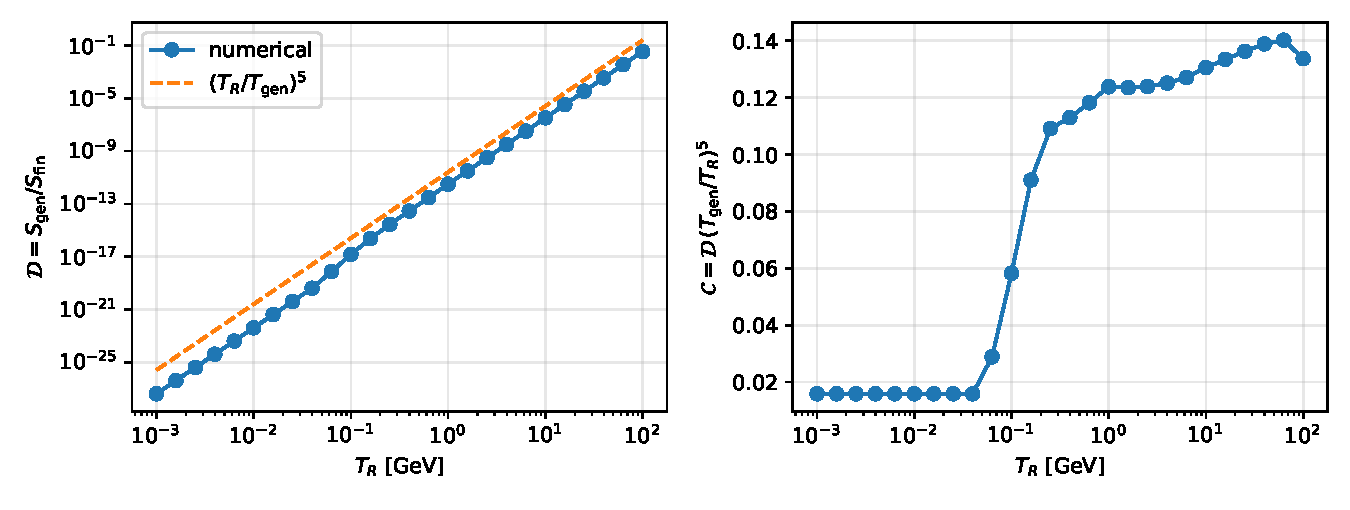
\includegraphics[width=.9\textwidth]{fig_dilution.pdf}
\caption{Entropy dilution $\mathcal D=S(\Tgen)/S_{\rm fin}$ for $\Tgen=131.7$~GeV from the numerical solution of \eqref{eq:boltz} (left) and the prefactor $\mathcal C=\mathcal D(\Tgen/T_R)^5$ (right). The step in $\mathcal C$ near $T_R\sim0.1$~GeV is the change of $g_*$ across the QCD crossover in our approximate $g_*(T)$.}\label{fig:dil}
\end{figure}

\section{Electroweak sphalerons in an EMDE}\label{sec:sph}
\subsection{Susceptibility}
Sphaleron transitions change Chern--Simons number by $\Delta N_{\rm CS}=\pm1$ and create twelve left-handed doublet fermions (nine quarks and three leptons). A bias $\mu_{\rm CS}$ conjugate to $N_{\rm CS}$ therefore enforces $n_g(3\mu_Q+\mu_L)=\mu_{\rm CS}$ in sphaleron equilibrium. Imposing Yukawa equilibrium ($\mu_u=\mu_Q+\mu_H$, $\mu_d=\mu_Q-\mu_H$, $\mu_e=\mu_L-\mu_H$), hypercharge neutrality, and number densities $n=\tfrac{T^2}{6}g\mu$ (fermions) and $\tfrac{T^2}{3}g\mu$ (bosons), we solve the linear system symbolically (Appendix~\ref{app:xi}). For $B-L=0$,
\begin{equation}
n_B=\frac{12}{79}\,T^2\mu_{\rm CS}\ \Rightarrow\ Y_B=\xi\,\frac{\mu_{\rm CS}}{T},\qquad \xi=\frac{12/79}{2\pi^2g_*/45}=\xiv,\label{eq:xi}
\end{equation}
while for $\mu_{\rm CS}=0$ the same system reproduces the standard $B=\tfrac{28}{79}(B-L)$, which checks the setup.

\subsection{Rate and equilibrium window}
The lattice sphaleron rate for $m_H=125$~GeV is \cite{DRT:2014}
\begin{equation}
\frac{\Gamma_{\rm sph}}{T^4}=\begin{cases}\exp(0.83\,T/\text{GeV}-147.7), & 130~\text{GeV}<T<T_c,\\ 18\,\alpha_W^5,& T>T_c,\end{cases}\qquad T_c=159~\text{GeV},\label{eq:rate}
\end{equation}
and in radiation domination the freeze-out temperature, where $\Gamma_{\rm sph}\sim H$, is $T_*=131.7\pm2.3$~GeV. We encode the criterion as $\Gamma_{\rm sph}/T^3\ge c\,H$ with $c=\ccal$ fixed to reproduce $T_*=131.7$~GeV in radiation domination; the lattice paper \cite{DRT:2012} notes freeze-out when the rate is about ten times $H$, consistent with $1/c\simeq8.5$ being the relaxation coefficient used below. In an EMDE $H$ is given by \eqref{eq:HEMDE} and grows as $T^4$, while $\Gamma_{\rm sph}/T^3$ grows only as $T$ above $T_c$. Equilibrium holds only in a window
\begin{equation}
T_*(T_R)<T<T_{\rm up}(T_R),\qquad T_{\rm up}^3=\frac{18\alpha_W^5T_R^2\MP}{c\,\kappa}.\label{eq:window}
\end{equation}
The scaling of the upper edge, $T_{\rm up}\propto T_R^{2/3}$, was obtained in Ref.~\cite{DLR:2000} with a perturbative rate; here the lattice rate fixes its coefficient and the broken-phase fit fixes the lower edge. Fig.~\ref{fig:win} and Table~\ref{tab:win} give the result. The lower edge moves from $131.7$~GeV toward $T_c$ as $T_R$ decreases, and the window closes entirely for $T_R\lesssim\TReqc$~MeV ($\TReqlo$--$\TReqhi$~MeV for $c\to c/10,10c$), i.e.\ at or below the BBN bound.

\begin{figure}[t]
\centering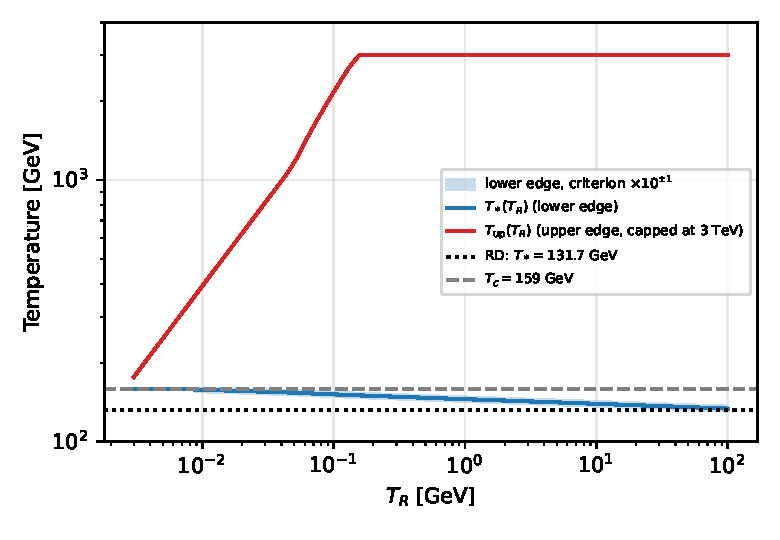
\includegraphics[width=.6\textwidth]{fig_window.pdf}
\caption{Temperature window in which electroweak sphalerons are in equilibrium during an EMDE. The band shows the sensitivity of the lower edge to the freeze-out criterion.}\label{fig:win}
\end{figure}
\begin{table}[t]
\centering
\begin{tabular}{r|cccc}
\toprule
$T_R$ & 18 MeV & 56 MeV & 1 GeV & 10 GeV\\
\midrule
$T_*$ [GeV] & \Tstara & \Tstarb & \Tstarc & \Tstard\\
$T_{\rm up}$ [GeV] & \Tupa & \Tupb & $\Tupc$ & $\Tupd$\\
\bottomrule
\end{tabular}
\caption{Sphaleron equilibrium window for representative $T_R$.}\label{tab:win}
\end{table}

\subsection{Full washout Boltzmann system}\label{sec:washout}
Let each modulus decay create baryon number $\epsilon_B$ and lepton number $\epsilon_L$. With comoving densities $N_X=n_Xa^3$ and $N_\phi=\rho_\phi a^3/m$,
\begin{align}
\dot N_{B-L}&=(\epsilon_B-\epsilon_L)\,\Gamma N_\phi,\nonumber\\
\dot N_B&=\epsilon_B\,\Gamma N_\phi-\lambda_{\rm sph}(T)\Big(N_B-\tfrac{28}{79}N_{B-L}\Big),\qquad \lambda_{\rm sph}=\frac{1}{c}\frac{\Gamma_{\rm sph}}{T^3},\label{eq:washout}
\end{align}
solved together with \eqref{eq:boltz}. The relaxation target $\tfrac{28}{79}N_{B-L}$ is the symmetric-phase value; the change to the broken-phase coefficient near freeze-out is a few-percent effect that we neglect. Because \eqref{eq:washout} is linear in the sources, the final baryon number is $N_B^{\rm fin}=\eta_B\epsilon_B N_\phi^{\rm tot}$ (for $\epsilon_L=0$) and $N_B^{\rm fin}=-\eta_L\epsilon_LN_\phi^{\rm tot}$ (for $\epsilon_B=0$), with efficiencies depending only on $T_R$. Fig.~\ref{fig:eta} shows the result.

\begin{figure}[t]
\centering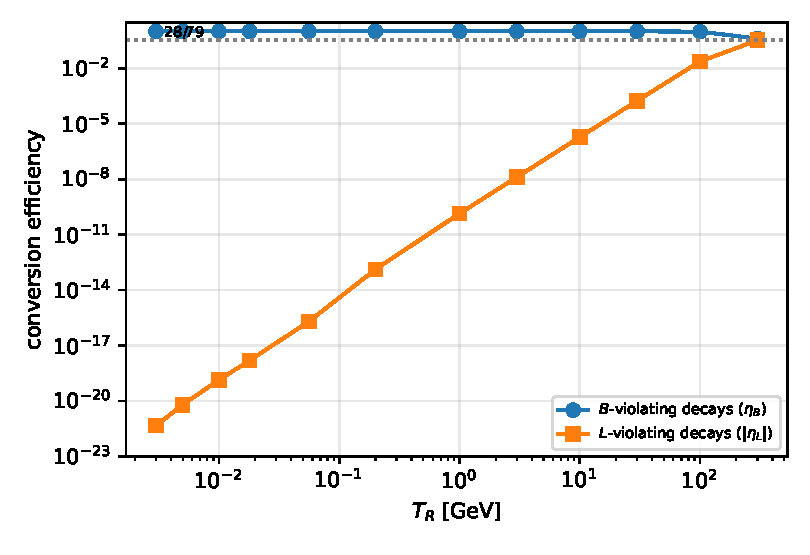
\includegraphics[width=.62\textwidth]{fig_eta.pdf}
\caption{Conversion efficiencies from the full washout Boltzmann system \eqref{eq:washout}. $B$-violating decays survive intact for $T_R\lesssim30$~GeV; lepton asymmetries are converted only if a non-negligible fraction of the modulus decays while sphalerons are in equilibrium.}\label{fig:eta}
\end{figure}

For $T_R\lesssim30$~GeV, $\eta_B=1$ to better than $10^{-3}$: baryon number created in the decay is left untouched because sphalerons have decoupled before the bulk of the decays. For larger $T_R$ it falls to $\etaBc$ at $T_R=100$~GeV and $\etaBd$ at $300$~GeV, approaching $28/79$. The lepton channel behaves oppositely. Only the fraction $f_{\rm win}\simeq\tfrac23\Gamma/H(T_*)\propto T_R^4$ of the modulus decays while sphalerons are active, giving $\eta_L\simeq\tfrac{28}{79}f_{\rm win}$ (e.g.\ $\etaLa$ at 18~MeV and $\etaLb$ at 1~GeV, matching the numerical solution) and $\eta_L\simeq\etaLone\,(T_R/\mathrm{GeV})^{\etaLexp}$ in the range $1$--$10$~GeV, reaching $\etaLd$ at 100~GeV and $\etaLe$ at 300~GeV. Hence \emph{leptogenesis from modulus decay requires $T_R\gtrsim100$--$300$~GeV}, and for any $T_R\lesssim30$~GeV the sphalerons are spectators.
\begin{proposition}[Closed forms]\label{prop:closed}
In the steady-state regime \eqref{eq:HEMDE}:
\begin{enumerate}
\item[(i)] the sphaleron window closes when $T_{\rm up}=T_c$, i.e.\ at $T_R^{\rm eq}=\big(c\,\kappa\,T_c^3/18\alpha_W^5\MP\big)^{1/2}=\TReqclosed$~MeV, in agreement with the numerical value $\TReqc$~MeV;
\item[(ii)] for $T_R\ll T_*$ the lepton-to-baryon conversion efficiency is
\begin{equation}
\eta_L\simeq\frac{28}{79}\cdot\frac23\frac{\Gamma}{H(T_*)}=\frac{28}{79}\,\frac{4}{15}\,\frac{g_R}{g_*}\Big(\frac{T_R}{T_*}\Big)^4,\label{eq:etaclosed}
\end{equation}
giving $\etaClosedA$, $\etaClosedB$, $\etaClosedC$ for $T_R=18$~MeV, 1~GeV, 10~GeV, within $10\%$ of the numerical solution of \eqref{eq:washout};
\item[(iii)] baryon-violating decays are processed only by the same fraction, $\eta_B\simeq1-\tfrac{51}{79}\cdot\tfrac23\Gamma/H(T_*)=1-\mathcal O(\eta_L)$.
\end{enumerate}
\end{proposition}
\begin{proof}
(i) Equate \eqref{eq:window} to $T_c$. (ii) The fraction of the modulus energy that has decayed by cosmic time $t=2/3H$ is $\Gamma t=\tfrac23\Gamma/H$; B$-$L produced before sphaleron freeze-out is converted with coefficient $28/79$ and all later decays leave $B$ untouched. Using \eqref{eq:TR} and \eqref{eq:HEMDE}, $\Gamma/H=36\,\Gamma^2\MP^2/(\pi^2g_*T^4)=\tfrac{2g_R}{5g_*}(T_R/T)^4$. (iii) Early-produced baryon number relaxes to $\tfrac{28}{79}$ of its $B-L$.
\end{proof}
\noindent\emph{Remark.} Multiplying \eqref{eq:etaclosed} by the decay yield $\epsilon\kappa_YT_R/m$ gives $Y_B\propto\epsilon\,T_R^5/(T_*^4m)$, which has the scaling of the suppression found for non-thermal leptogenesis in Ref.~\cite{GHKO:2026}.


\section{Which sources can work}\label{sec:sources}
\subsection{Anomaly-induced chemical potentials are frame independent}
Let $\theta^i=a^i/f$ be axion angles with $L_{\rm kin}=\tfrac12G_{ij}\dot\theta^i\dot\theta^j$ ($G_{ij}$ of dimension mass$^2$, constant at the vacuum) coupled to the electroweak gauge fields via
\begin{equation}
\mathcal L\supset\frac{g^2}{32\pi^2}\,c_i\,\theta^i\,W^a_{\mu\nu}\widetilde W^{a\,\mu\nu},\qquad c_i=\text{const}.\label{eq:anom}
\end{equation}
In string compactifications $c_i=k_i$ are the integer coefficients of the holomorphic gauge kinetic function $f_W=k_iT^i$, which are not renormalised by thermal effects. Since $\tfrac{g^2}{32\pi^2}W\widetilde W=\partial_\mu K^\mu$, integration by parts gives
\begin{equation}
\mu_{\rm CS}=\frac{\dd}{\dd t}\big(c_i\theta^i\big)=c_i\dot\theta^i.
\end{equation}
\begin{proposition}[Frame independence]\label{prop:frame}
Let $\tilde\theta^\alpha=R^\alpha{}_i(t)\theta^i$ with $R(t)\in SO(n)$ an arbitrary time-dependent change of basis and $\tilde c_\alpha(t)=c_iR_\alpha{}^{\,i}$, so that $c_i\theta^i=\tilde c_\alpha\tilde\theta^\alpha$. Then
\begin{equation}
\mu_{\rm CS}=\tilde c_\alpha\dot{\tilde\theta}^\alpha+\dot{\tilde c}_\alpha\tilde\theta^\alpha=c_i\dot\theta^i .
\end{equation}
In particular if $\dot\theta^i=0$ then $\mu_{\rm CS}=0$ for every $R(t)$: the rotating-frame velocity $\dot{\tilde\theta}^\alpha=\dot R^\alpha{}_i\theta^i\neq0$ is exactly cancelled by $\dot{\tilde c}_\alpha\tilde\theta^\alpha$.
\end{proposition}
\begin{proof}
Differentiate $c_i\theta^i=\tilde c_\alpha(t)\tilde\theta^\alpha$ with the product rule; the left side is $c_i\dot\theta^i$ because $c_i$ is constant.
\end{proof}
\noindent\emph{Example.} For $\theta=(\theta_0,0)$ frozen and $c=(N,0)$, rotate by $\vartheta(t)$: $\tilde\theta_L=\theta_0\sin\vartheta$, $\tilde\theta_\perp=\theta_0\cos\vartheta$, $\tilde c=(N\sin\vartheta,N\cos\vartheta)$. Then $\tilde c_L\dot{\tilde\theta}_L=N\theta_0\dot\vartheta\sin\vartheta\cos\vartheta=-\tilde c_\perp\dot{\tilde\theta}_\perp$, so the sum vanishes, whereas the projection onto the rotating direction alone, $N\dot{\tilde\theta}_L=N\theta_0\dot\vartheta\cos\vartheta$, does not. (Verified symbolically.)
\begin{corollary}
Rotations of the eigenbasis of any operator acting on the moduli, including avoided crossings in a thermal mass matrix, generate no $\mu_{B+L}$ unless the axions acquire a coordinate velocity $\dot\theta^i\neq0$.
\end{corollary}

\subsection{A universal bound on axion-driven baryogenesis}
Define the effective anomalous decay constant
\begin{equation}
F\equiv\big(c_iG^{ij}c_j\big)^{-1/2},\label{eq:F}
\end{equation}
which for a single axion with $\theta=a/f$ is $F=f/N$.
\begin{theorem}[Kinetic-energy bound]\label{thm:axion}
Let sphalerons be in equilibrium at $T_{\rm gen}$ and let $\rho_{\rm kin}=\tfrac12G_{ij}\dot\theta^i\dot\theta^j\le\rho_{\rm tot}=3H^2\MP^2$. Then
\begin{equation}
\frac{\mu_{\rm CS}}{T}\le\frac{\sqrt6\,H\MP}{F\,T},\qquad Y_B^{\rm gen}\le\xi\,\frac{\sqrt6\,H(\Tgen)\MP}{F\,\Tgen}.\label{eq:kin}
\end{equation}
In radiation domination $H=\sqrt{\pi^2g_*/90}\,T^2/\MP$ and this becomes
\begin{equation}
Y_B^{\rm gen}\le\xi\,\pi\sqrt{\frac{g_*}{15}}\,\frac{\Tgen}{F}\simeq\frac{3.6~\text{GeV}}{F},\qquad\text{so that}\quad F\le F_{\max}=\fNmax~\text{GeV}\label{eq:Fmax}
\end{equation}
is necessary to reach $\Yobs=8.6\times10^{-11}$.
\end{theorem}
\begin{proof}
By Cauchy--Schwarz in the metric $G$, $|c_i\dot\theta^i|=|c_iG^{ij}(G_{jk}\dot\theta^k)|\le\sqrt{c_iG^{ij}c_j}\,\sqrt{G_{kl}\dot\theta^k\dot\theta^l}=F^{-1}\sqrt{2\rho_{\rm kin}}\le F^{-1}\sqrt{6}\,H\MP$. Sphaleron equilibrium gives $Y_B=\xi\mu_{\rm CS}/T$ by \eqref{eq:xi}; if $\mu_{\rm CS}$ varies faster than the relaxation rate $\lambda_{\rm sph}$ the response is smaller, so \eqref{eq:xi} is an upper bound. Evaluating at $T_{\rm gen}=131.7$~GeV, $g_*=106.75$, $\xi=\xiv$ gives \eqref{eq:Fmax}.
\end{proof}
The bound requires no knowledge of the source dynamics: it holds for slow rotation, a first-order hidden-sector transition, or kination, and it is saturated only if the axion kinetic energy equals the total energy density. Because only the sphaleron freeze-out region contributes ($B+L$ relaxes to equilibrium while sphalerons are active, and $B-L$ is not generated by $\mu_{\rm CS}$), $T_{\rm gen}=T_*(T_R)$.

\paragraph{EMDE.} Including the dilution \eqref{eq:dil}, the final asymmetry obeys $Y_B^{\rm fin}\le\xi\sqrt6\,(H_{\rm EMDE}/T)(\MP/F)\,\mathcal D\propto T_R^{-2}\cdot T_R^5=T_R^3$, monotonic in $T_R$, so the best case is no EMDE. Numerically, for $T_R\le30$~GeV the maximal yield is reduced by a factor $\axEMDEratio$ relative to \eqref{eq:Fmax}, i.e.\ $F_{\max}\to2\times10^{8}$~GeV.

\paragraph{Relation to axiogenesis.} With $n_\theta=f^2\dot\theta$ the PQ charge density and $Y_\theta=n_\theta/s$, \eqref{eq:xi} gives for a single axion
\begin{equation}
Y_B=c_B\,N\,\frac{T^2}{f^2}\,Y_\theta,\qquad c_B=\frac{12}{79},\label{eq:axiogenesis}
\end{equation}
the relation underlying axiogenesis \cite{Co:2019}. Thm.~\ref{thm:axion} is \eqref{eq:axiogenesis} combined with $\rho_{\rm kin}\le\rho_{\rm tot}$, and is stated for several axions in terms of $F$. The version below adds the dark-matter requirement.
\begin{theorem}[Dark-matter-constrained bound]\label{thm:dm}
Suppose the rotation ends as cold, stable axion dark matter with conserved PQ charge and no dissipation after $T_{\rm gen}$, so that $m_a\,Y_\theta^{\rm fin}\le\rho_{\rm DM}/s=4.4\times10^{-10}$~GeV with $Y_\theta^{\rm fin}=\mathcal D\,Y_\theta^{\rm gen}$. Then, for any EMDE history,
\begin{equation}
Y_B^{\rm fin}=\mathcal D\,c_BN\frac{T_{\rm gen}^2}{f^2}Y_\theta^{\rm gen}\le c_BN\frac{T_{\rm gen}^2}{f^2}\frac{\rho_{\rm DM}/s}{m_a}\ \ \Longrightarrow\ \ \frac{f^2m_a}{N}\le\frac{c_B\,T_{\rm gen}^2\,(\rho_{\rm DM}/s)}{\Yobs}=\DMbound~\text{GeV}^3,
\end{equation}
independent of $\mathcal D$ because baryons and axion dark matter are diluted equally.
\end{theorem}
\noindent For the QCD axion ($m_af\simeq5.7\times10^{-3}$~GeV$^2$) this gives $f\lesssim2\times10^{6}N$~GeV, of the order of the bounds quoted in the axiogenesis literature ($f\lesssim10^{7}$--$10^{8}$~GeV) up to the $\mathcal O(1)$ conventions for $c_B$ and the kinetic-misalignment abundance. The bound can be evaded by dissipating the rotation \cite{Asadi:2025}, which is why Thm.~\ref{thm:axion} (which assumes nothing about the endpoint) is the robust statement.
\begin{proposition}[Classification of axions by mass and lifetime]\label{prop:class}
Let $H_*\equiv H(T_*)$ and let the axion have mass $m_a$ and decay rate $\Gamma_a$.
\begin{enumerate}
\item[(A)] $m_a\lesssim H_*$: the field is frozen and $|\dot\theta|\lesssim H_*\theta$; the source is Hubble-limited and bounded as below.
\item[(B)] $m_a\gg H_*$, $\Gamma_a\ll H_*$: the axion oscillates with $\dot\theta\sim m_a\theta$ and is long lived; Thms.~\ref{thm:axion} and~\ref{thm:dm} apply.
\item[(C)] $\Gamma_a\gtrsim H_*$: the coherent amplitude is suppressed by $e^{-\Gamma_a t/2}$ with $t\simeq1/2H_*$, i.e.\ by $e^{-\Gamma_a/4H_*}$; no coherent velocity survives at sphaleron freeze-out.
\end{enumerate}
\end{proposition}
\noindent Case (C) is exact within the linear decay approximation: a decaying oscillation transfers its energy to radiation, so the chemical potential averages to zero thermally.

\paragraph{Slowly varying sources.} If the source is limited by the Hubble rate, $|c_i\dot\theta^i|\le\nu H$, then $Y_B\le\xi\nu H/T$. In radiation domination at $T=131.7$~GeV, $H/T=\HTRD$, so $\nu=30$ gives $Y_B\le\YRD$, short of $\Yobs$ by $\thetaneed$; an EMDE does not help (best $T_R\le50$~GeV: $\YEMDEbest$ for $\nu=30$). Such a source needs $\nu\gtrsim10^{8}$, far above what thermal evolution of a slowly rotating basis can provide, consistent with Prop.~\ref{prop:frame}.

\subsection{Generic bound on $T_R$ for pre-decay generation}
Let a mechanism act at $\Tgen$ with maximal chemical potential $(\mu/T)_{\max}$. Then $Y_B^{\rm fin}\le\mathcal D(T_R)\,\xi\,(\mu/T)_{\max}$ and
\begin{equation}
T_R\ge T_R^{\min}\simeq\Tgen\left[\frac{\Yobs}{\mathcal C\,\xi\,(\mu/T)_{\max}}\right]^{1/5}.\label{eq:TRmin}
\end{equation}
Evaluating with the numerical $\mathcal D$ (Fig.~\ref{fig:TRmin}):
\begin{center}
\begin{tabular}{c|ccccc}
\toprule
$(\mu/T)_{\max}$ & $1$ & $\muTb$ & $\muTc$ & $\muTd$ & $\muTe$\\
$T_R^{\min}$ [GeV] & $\TRmina$ & $\TRminb$ & $\TRminc$ & $\TRmind$ & $\TRmine$\\
\bottomrule
\end{tabular}
\end{center}
Since $\mathcal D\propto\Tgen^{-5}$, $T_R^{\min}\propto\Tgen$.
\begin{figure}[t]
\centering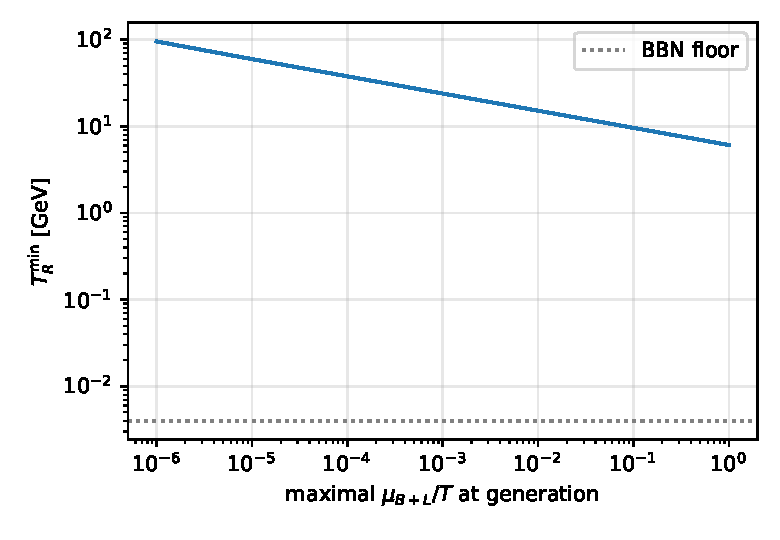
\includegraphics[width=.55\textwidth]{fig_TRmin.pdf}
\caption{Minimal reheating temperature for a pre-decay asymmetry generated at $\Tgen=131.7$~GeV as a function of the maximal chemical potential reached.}\label{fig:TRmin}
\end{figure}

\section{Application to Large Volume Scenarios}\label{sec:lvs}
\subsection{Explicit vacua}\label{sec:explicit}
We use the Swiss-cheese compactification on $\mathbb P^4_{[1,1,1,6,9]}$ ($h^{1,1}=2$, $\chi=-540$) \cite{Balasubramanian:2005zx}:
\begin{equation}
K=-2\ln\big(\mathcal V+\tfrac{\hat\xi}{2}\big),\quad\mathcal V=\gamma(\tau_b^{3/2}-\tau_s^{3/2}),\quad\gamma=\tfrac{1}{9\sqrt2},\quad\hat\xi=\frac{-\zeta(3)\chi}{2(2\pi)^3g_s^{3/2}},\quad W=W_0+Ae^{-aT_s},\label{eq:swiss}
\end{equation}
with $W_0=1$, $|A|=1$ (sign chosen such that the $T_s$--$W_0$ cross term is negative), $a=2\pi/N$ treated as a continuous parameter, and $g_s=0.3$ (0.4 for the smallest volumes). We evaluate the exact $\mathcal N=1$ potential $V=e^K(K^{i\bar j}D_iW\overline{D_jW}-3|W|^2)$ at $110$ digits, locate the minimum by nested one-dimensional minimisation seeded from the reduced three-term potential and refined by Newton iteration, verify that the Hessian in $(\tau_b,\tau_s,\mathrm{Im}\,T_s)$ is positive definite, and canonically normalise with $G_{ij}=2\MP^2K_{i\bar j}$ (Appendix~\ref{app:vac}). An AdS minimum exists only if $\tau_s^{3/2}\gtrsim3\hat\xi/8\gamma$, which fixes the allowed $g_s$. Table~\ref{tab:explicit} lists ten vacua covering $\mathcal V=2.5\times10^3$--$10^{16}$.
\begin{table}[t]
\centering\small
\begin{tabular}{c|ccccc}
\toprule
$\mathcal V$ & $\tau_s$ & $m_{3/2}$ [GeV] & $m_{\tau_b}$ [GeV] & $m_{\tau_s}\simeq m_\rho$ [GeV] & $T_R$ [GeV]\\
\midrule
$1.0\times10^{16}$ & $13.8$ & $2.4\times10^{2}$ & $2.4\times10^{-6}$ & $1.9\times10^{4}$ & $6.4\times10^{-19}$ \\
$4.3\times10^{14}$ & $13.8$ & $5.7\times10^{3}$ & $2.9\times10^{-4}$ & $4.1\times10^{5}$ & $8.6\times10^{-16}$ \\
$8.9\times10^{12}$ & $13.8$ & $2.7\times10^{5}$ & $1.0\times10^{-1}$ & $1.7\times10^{7}$ & $5.6\times10^{-12}$ \\
$4.1\times10^{11}$ & $13.9$ & $5.9\times10^{6}$ & $1.1\times10^{1}$ & $3.4\times10^{8}$ & $6.2\times10^{-9}$ \\
$7.9\times10^{9}$ & $13.9$ & $3.1\times10^{8}$ & $4.4\times10^{3}$ & $1.5\times10^{10}$ & $5.0\times10^{-5}$ \\
$4.2\times10^{8}$ & $13.9$ & $5.8\times10^{9}$ & $3.8\times10^{5}$ & $2.5\times10^{11}$ & $4.1\times10^{-2}$ \\
$7.1\times10^{6}$ & $14.0$ & $3.4\times10^{11}$ & $2.0\times10^{8}$ & $1.2\times10^{13}$ & $2.7\times10^{2}$ \\
$4.8\times10^{5}$ & $14.0$ & $5.1\times10^{12}$ & $1.2\times10^{10}$ & $1.5\times10^{14}$ & $1.3\times10^{5}$ \\
$1.8\times10^{4}$ & $14.1$ & $1.4\times10^{14}$ & $2.0\times10^{12}$ & $3.0\times10^{15}$ & $2.7\times10^{8}$ \\
$2.5\times10^{3}$ & $14.3$ & $9.6\times10^{14}$ & $4.0\times10^{13}$ & $1.6\times10^{16}$ & $2.5\times10^{10}$ \\
\bottomrule
\end{tabular}
\caption{Explicit Swiss-cheese vacua. $T_R$ is computed from $\Gamma=m_{\tau_b}^3/(4\pi\MP^2)$ ($c_\Gamma=1$) via \eqref{eq:TR}; $m_{\tau_s}\simeq m_\rho\simeq(17\text{--}78)\,m_{3/2}$. Entries with $T_R\gtrsim T_*$ correspond to no EMDE at the electroweak scale and are given only for completeness.}\label{tab:explicit}
\end{table}
The results confirm the parametric scalings $m_{3/2}\simeq\MP/\mathcal V$ and $m_{\tau_b}=c_m\MP\mathcal V^{-3/2}$ with $c_m=\cmmin$--$\cmmax$ (decreasing towards large $\mathcal V$), so that a modulus mass of $10^5$~GeV corresponds to $\mathcal V\sim10^9$, not $10^{15}$.

\paragraph{Decay width and dark radiation.} The width into the bulk axion partner is universal, $\Gamma_{aa}=m_{\tau_b}^3/(48\pi\MP^2)$ \cite{Cicoli:2012}, i.e.\ it contributes $c_\Gamma=1/12$ to $\Gamma=c_\Gamma m_{\tau_b}^3/(4\pi\MP^2)$ and produces dark radiation; $\Delta N_{\rm eff}=\tfrac{43}{7}(10.75/g_*(T_d))^{1/3}B_a/(1-B_a)$ \cite{Higaki:2012} with $\Delta N_{\rm eff}<0.3$ requires $B_a\lesssim\Bamaxa$ ($T_R\sim\mathrm{MeV}$) to $\Bamaxb$ ($T_R\sim10$~GeV), hence $c_\Gamma\gtrsim\cGminb$--$\cGmina$. We take $c_\Gamma=1$ as benchmark and vary it from $0.3$ to $8$.

\subsection{K3-fibred vacua: the fibre-inflation model}\label{sec:k3}
We take the K3-fibred geometry $\mathcal V=\alpha(\sqrt{\tau_1}\tau_2-\gamma\tau_3^{3/2})$ of Cicoli, Burgess and Quevedo \cite{Cicoli:2008}, in which $\tau_1$ is the K3-fibre divisor, $\tau_2$ the base-type divisor and $\tau_3$ a blow-up. Tree-level, $\alpha'$ and non-perturbative terms stabilise $\mathcal V$ and $\tau_3$ as in Sec.~\ref{sec:explicit} and leave $\tau_1$ at fixed $\mathcal V$ exactly flat; this direction is lifted by string-loop corrections, which in the large-volume expansion give \cite{Cicoli:2008}
\begin{equation}
V=\mu_1\frac{\sqrt{\tau_3}}{\mathcal V}e^{-2a_3\tau_3}-\mu_2W_0\frac{\tau_3}{\mathcal V^2}e^{-a_3\tau_3}+\mu_3\frac{W_0^2}{\mathcal V^3}+\frac{\delta_{\rm up}}{\mathcal V^{4/3}}+\Big(\frac{A}{\tau_1^2}-\frac{B}{\mathcal V\sqrt{\tau_1}}+\frac{C\tau_1}{\mathcal V^2}\Big)\frac{W_0^2}{\mathcal V^2},\label{eq:k3pot}
\end{equation}
with $\mu_1=8a_3^2A_3^2/3\alpha\gamma$, $\mu_2=4a_3A_3$, $\mu_3=3\hat\xi/4$, $A=(g_sC_1^{KK})^2$, $B=4\alpha C_{12}^W$, $C=2(\alpha g_sC_2^{KK})^2$, and an overall normalisation $g_se^{K_{cs}}/8\pi$ with $K_{cs}=3\ln g_s$. The loop functional form is a conjecture based on a torus computation and low-energy arguments rather than an explicit Calabi--Yau computation \cite{Cicoli:2008}; we take it as given and use the coefficient sets published there. The warped uplift $\delta_{\rm up}$ is fixed by requiring a Minkowski vacuum.

We solve $\partial V=0=V$ at 60 digits in $(\tau_1,\mathcal V,\tau_3,\delta_{\rm up})$ and compute the mass matrix with the exact leading-order Kähler metric $K_{i\bar j}$ transformed to $(\tau_1,\mathcal V,\tau_3)$ (Appendix~\ref{app:k3}). Table~\ref{tab:k3sets} gives the three published parameter sets (LV, SV1, SV2). For LV, the numerical fibre-mass eigenvalue equals the analytic result of \cite{Cicoli:2008}, $m_f^2=4(1+\tfrac76R)C_2/\mathcal V^{10/3}$, to fourteen digits, which checks the implementation; $\mathcal V$, $\tau_3$ and $\tau_1$ differ from the tabulated values by $\lesssim50\%$, $\lesssim2\%$ and $\lesssim30\%$.
\begin{table}[t]
\centering\scriptsize
\begin{tabular}{l|ccccccc}
\toprule
Set & $\mathcal V$ & $\tau_1$ & $\tau_3$ & $m_{3/2}$ [GeV] & $m_f$ [GeV] & $m_{\tau_b}$ [GeV] & $m_{\tau_3}$ [GeV]\\
\midrule
LV & $4.2\times10^{13}$ & $1.4\times10^{6}$ & $10.6$ & $1.2\times10^{2}$ & $1.6\times10^{-6}$ & $1.8\times10^{-5}$ & $7.5\times10^{3}$ \\
SV1 & $1.2\times10^{3}$ & $7.0\times10^{0}$ & $4.3$ & $3.7\times10^{15}$ & $4.7\times10^{13}$ & $2.5\times10^{14}$ & $1.5\times10^{16}$ \\
SV2 & $9.4\times10^{2}$ & $5.2\times10^{0}$ & $3.5$ & $4.7\times10^{15}$ & $9.7\times10^{13}$ & $3.0\times10^{14}$ & $2.0\times10^{16}$ \\
\bottomrule
\end{tabular}
\caption{Published K3-fibred parameter sets \cite{Cicoli:2008}, solved as described in the text (with the normalisation $g_se^{K_{cs}}/8\pi$). The LV set has $m_{3/2}=\mathcal O(100)$~GeV and a fibre modulus of 1.6~keV.}\label{tab:k3sets}
\end{table}

To obtain the volume dependence we vary $a_3$ at fixed loop data of SV1 and fix $W_0$ such that $m_{3/2}=\MP/\mathcal V$ (the same normalisation as the Swiss-cheese scan). The fibre mass obeys the exact scaling
\begin{equation}
m_f=c_f\,\MP\,\mathcal V^{-5/3},\qquad m_{\tau_b}=c_m\,\MP\mathcal V^{-3/2}\quad(c_m=0.87\text{--}2.1),\label{eq:k3scaling}
\end{equation}
with $c_f=1.446$ constant to four digits over $\mathcal V=10^3$--$10^{10}$. Varying the loop data by factors of three gives $c_f=0.70$ ($B/3$), $1.20$ ($A\times3$, $C\times9$) and $3.01$ ($B\times3$), and the published LV loop data give $c_f=17$ (in units of $m_{3/2}\mathcal V^{-2/3}$). The fibre modulus is therefore the lightest modulus for all of these, and $T_R\propto\MP\mathcal V^{-5/2}$ (Fig.~\ref{fig:TRV}). Table~\ref{tab:k3} gives the resulting bounds.
\begin{figure}[t]
\centering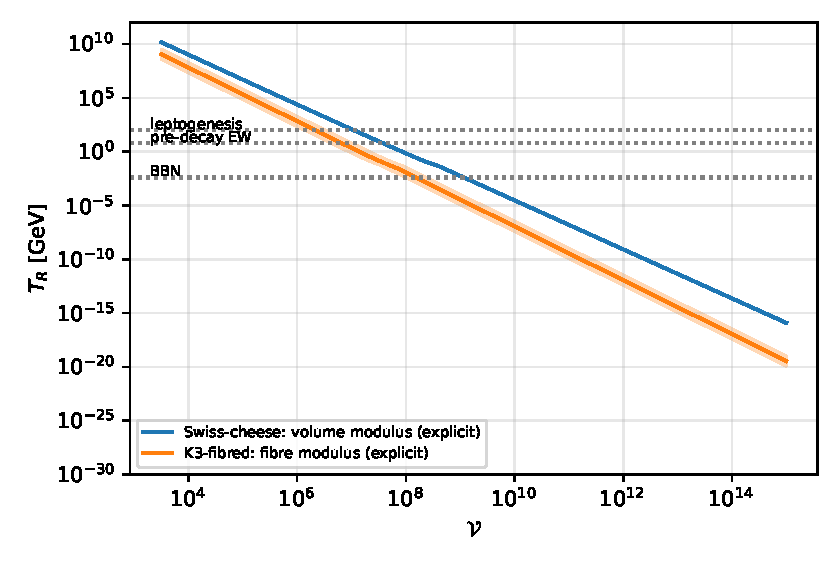
\includegraphics[width=.62\textwidth]{fig_TRV.pdf}
\caption{Reheating temperature set by the lightest modulus as a function of volume: the volume modulus in the explicit Swiss-cheese vacua (blue) and the fibre modulus in the explicit K3-fibred vacua (orange band: $c_f=0.7$--$3$). Dotted lines mark the BBN bound and the pre-decay electroweak and decay-leptogenesis requirements.}\label{fig:TRV}
\end{figure}
\begin{table}[t]
\centering\scriptsize
\begin{tabular}{l|cccccc}
\toprule
Geometry & $T_R\ge6.1$~GeV & $T_R\ge100$~GeV & $T_R\ge4$~MeV & $\epsilon=1$ & $\epsilon=10^{-2}$ & $\epsilon=10^{-4}$\\
\midrule
Swiss-cheese (explicit vacua) & $3.8\times10^{7}$ & $1.1\times10^{7}$ & $1.2\times10^{9}$ & $3.1\times10^{12}$ & $7.3\times10^{9}$ & $2.6\times10^{6}$ \\
K3-fibred, $c_f=0.7$ & $4.3\times10^{6}$ & $1.4\times10^{6}$ & $9.8\times10^{7}$ & $1.3\times10^{11}$ & $5.3\times10^{8}$ & $3.6\times10^{5}$ \\
K3-fibred, $c_f=1.45$ (reference) & $6.6\times10^{6}$ & $2.1\times10^{6}$ & $1.5\times10^{8}$ & $2.0\times10^{11}$ & $8.1\times10^{8}$ & $5.6\times10^{5}$ \\
K3-fibred, $c_f=3.0$ & $1.0\times10^{7}$ & $3.3\times10^{6}$ & $2.4\times10^{8}$ & $3.2\times10^{11}$ & $1.3\times10^{9}$ & $8.7\times10^{5}$ \\
K3-fibred, $c_f=17.1$ (CBQ LV loop data) & $2.9\times10^{7}$ & $9.4\times10^{6}$ & $6.7\times10^{8}$ & $9.0\times10^{11}$ & $3.6\times10^{9}$ & $2.5\times10^{6}$ \\
\bottomrule
\end{tabular}
\caption{Upper bounds on $\mathcal V$ from explicit vacua: pre-decay electroweak baryogenesis ($T_R\ge6.1$~GeV), decay leptogenesis ($T_R\ge100$~GeV), BBN ($T_R\ge4$~MeV), and $B$-violating decays for CP-violating baryon number $\epsilon$ per decay. K3 rows use \eqref{eq:k3scaling}.}\label{tab:k3}
\end{table}
All bounds tighten by roughly an order of magnitude relative to the Swiss-cheese case: $\mathcal V\lesssim7\times10^6$ for pre-decay electroweak baryogenesis at the reference $c_f$, and the BBN requirement alone gives $\mathcal V\lesssim10^8$. If heavier moduli (the volume modulus and $\tau_3$) decay earlier, the universe returns to radiation domination before the fibre modulus dominates again; this inserts additional dilution but cannot increase the final asymmetry, so the yields computed above are upper bounds for multi-stage histories. For the published TeV-scale LV set ($\mathcal V=4\times10^{13}$) the fibre modulus has $T_R\simeq4\times10^{-19}$~GeV, the standard LVS cosmological moduli problem, and the volume modulus is $18$~keV.

\subsection{Channel by channel}
\paragraph{(a) Pre-decay electroweak baryogenesis.} By \eqref{eq:TRmin}, $T_R\gtrsim6$--$38$~GeV, which in the explicit vacua means $\mathcal V\lesssim\VexpTRa$ ($T_R\ge6.1$~GeV) to $\VexpTRb$ ($T_R\ge38$~GeV), with $\VexpTRaLo$--$\VexpTRaHi$ for $c_\Gamma\in[0.3,8]$, and $m_{3/2}\gtrsim10^{10}$~GeV. For $\mathcal V=10^{16}$ the explicit vacuum has $T_R\simeq6\times10^{-19}$~GeV: excluded irrespective of mechanism.

\paragraph{(b) Axion-driven (Chern--Simons) baryogenesis.} The result depends on which cycle supports the electroweak gauge group.

\emph{Bulk or fibre cycle.} For $f_W=NT$ with $T$ a bulk or fibre modulus, $K_{T\bar T}=\mathcal O(1)/\tau^2$ and $\alpha_W^{-1}=N\tau$, so the axion decay constant (with $\theta=2\pi\,\mathrm{Im}\,T$ and $L_{\rm kin}=\MP^2K_{T\bar T}(\partial\,\mathrm{Im}\,T)^2$) is
\begin{equation}
F=\frac{f}{N}=\frac{\MP\sqrt{2K_{T\bar T}}}{2\pi N}=\kappa_F\,\frac{\alpha_W\MP}{4\pi},\qquad\kappa_F=2\tau\sqrt{2K_{T\bar T}}=\mathcal O(1),
\end{equation}
independent of $N$ and $\tau$ ($\kappa_F=\sqrt2$ for the fibre, $K_{T\bar T}=1/4\tau^2$). With $\alpha_W=0.034$,
\begin{equation}
F\simeq\fNLVS~\text{GeV}\ \ \Rightarrow\ \ Y_B^{\max}\simeq\Ymaxaxion,\qquad \frac{F}{F_{\max}}\simeq\fNshort.
\end{equation}
Thm.~\ref{thm:axion} therefore excludes every axion-velocity mechanism at the electroweak scale for such axions, including a first-order hidden-sector transition, by more than five orders of magnitude even at kination; an EMDE worsens this by $\sim200$.

\emph{Blow-up cycle.} If the Standard Model sits on a small blow-up cycle $\tau_s$ (Swiss-cheese geometry, $\mathcal V=\gamma(\tau_b^{3/2}-\tau_s^{3/2})$), the Kähler metric is volume suppressed,
\begin{equation}
K_{s\bar s}\simeq\frac{3\gamma}{8\sqrt{\tau_s}\,\mathcal V},\qquad F_s=\frac{\MP}{2\pi N}\sqrt{\frac{3\gamma}{4\sqrt{\tau_s}\,\mathcal V}}\simeq\frac{\FsCoef~\text{GeV}}{\sqrt{\mathcal V}}\quad(N\tau_s=\alpha_W^{-1},\ \gamma=1/9\sqrt2),
\end{equation}
(Appendix~\ref{app:K}), so $F_s$ \emph{does} satisfy Thm.~\ref{thm:axion} for $\mathcal V\gtrsim\Vthm$, including TeV-scale LVS. The axion is however heavy, $m_\rho\simeq(17\text{--}78)\,m_{3/2}$ in the explicit vacua, and decays to Standard Model gauge bosons with $\Gamma_\rho\simeq\tfrac38\alpha_W^2m_\rho^3/(32\pi^3F_s^2)$. Table~\ref{tab:fs} (explicit vacua, $N_{\rm SM}=\alpha_W^{-1}/\tau_s$) shows $\Gamma_\rho/H(T_*)\ge\GHminExp$ for all $\mathcal V$ from $2.5\times10^3$ to $10^{16}$, so it is in class (C) of Prop.~\ref{prop:class}: its oscillations are gone before sphaleron freeze-out and it provides no velocity. Thus the bound is not what excludes this case; its fast decay is.
\begin{table}[t]
\centering
\begin{tabular}{c|cc}
\toprule
$\mathcal V$ & $F_s$ [GeV] & $\Gamma_\rho/H(T_*)$\\
\midrule
$1.0\times10^{16}$ & $2.3\times10^{8}$ & $2.3\times10^{3}$ \\
$4.3\times10^{14}$ & $1.1\times10^{9}$ & $1.0\times10^{6}$ \\
$8.9\times10^{12}$ & $7.6\times10^{9}$ & $1.6\times10^{9}$ \\
$4.1\times10^{11}$ & $3.6\times10^{10}$ & $5.6\times10^{11}$ \\
$7.9\times10^{9}$ & $2.6\times10^{11}$ & $9.3\times10^{14}$ \\
$4.2\times10^{8}$ & $1.1\times10^{12}$ & $2.2\times10^{17}$ \\
$7.1\times10^{6}$ & $8.6\times10^{12}$ & $4.0\times10^{20}$ \\
$4.8\times10^{5}$ & $3.3\times10^{13}$ & $5.0\times10^{22}$ \\
$1.8\times10^{4}$ & $1.8\times10^{14}$ & $1.5\times10^{25}$ \\
$2.5\times10^{3}$ & $4.6\times10^{14}$ & $3.7\times10^{26}$ \\
\bottomrule
\end{tabular}
\caption{Blow-up-cycle axion in the explicit vacua of Table~\ref{tab:explicit}: decay constant $F_s=\MP\sqrt{2K_{s\bar s}}/2\pi N_{\rm SM}$ and decay rate $\Gamma_\rho$ into Standard Model gauge bosons relative to the Hubble rate at $T_*=131.7$~GeV ($H_*=\HTstar$~GeV).}\label{tab:fs}
\end{table}

\emph{Other axions.} Axions that are light and frozen (class A) are covered by the Hubble-limited bound; axions that are heavy and long lived (class B) by Thms.~\ref{thm:axion},~\ref{thm:dm}.

\paragraph{(c) Lepton-violating modulus decays.} By Sec.~\ref{sec:washout}, $\eta_L\simeq\etaLone(T_R/\mathrm{GeV})^{\etaLexp}$: for $T_R\lesssim30$~GeV the conversion is below $2\times10^{-4}$, so leptogenesis from modulus decay is impossible unless $T_R\gtrsim100$~GeV ($\mathcal V\lesssim\VexpTRlep$).

\paragraph{(d) Baryon-violating modulus decays.} With $\epsilon$ the CP-violating baryon number per decay, $Y_B=\epsilon\,\eta_B\,\kappa_Y\,T_R/m_{\tau_b}$ where the numerical solution gives $\kappa_Y\simeq0.7$--$0.9$ (sudden-decay value $3/4$). Using $T_R/m\propto\mathcal V^{-3/4}$ the bound scales as $\mathcal V_{\max}\propto\epsilon^{4/3}$; in the explicit vacua
\begin{equation}
\mathcal V_{\max}(\epsilon)=\VexpEpsone,\ \VexpEpstwo,\ \VexpEpsfour,\ \VexpEpssix\quad\text{for }\epsilon=1,\,10^{-2},\,10^{-4},\,10^{-6},
\end{equation}
shown in Fig.~\ref{fig:map}. TeV-scale LVS requires $\epsilon\gg1$ and is excluded; volumes $\mathcal V\sim10^{6}$--$10^{10}$ with $\epsilon\sim10^{-4}$--$10^{-2}$ remain viable.

\paragraph{(e) Affleck--Dine baryogenesis} is analysed in Sec.~\ref{sec:ad}; it provides the positive window for $\mathcal V\lesssim10^{6}$.

\begin{figure}[t]
\centering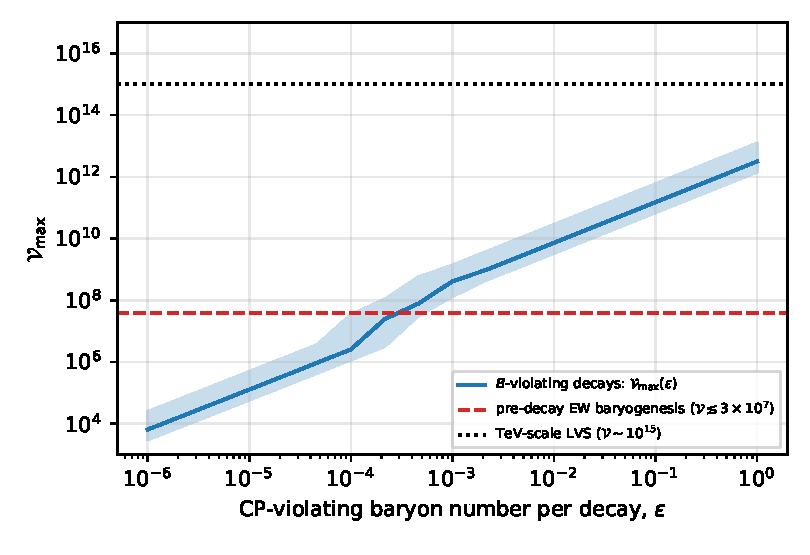
\includegraphics[width=.62\textwidth]{fig_map.pdf}
\caption{Maximum LVS volume allowed by $B$-violating modulus decays, $\mathcal V_{\max}(\epsilon)$ (explicit vacua; band: $c_\Gamma\in[0.3,8]$). The dashed line is the pre-decay electroweak bound; TeV-scale LVS lies at $\mathcal V\sim10^{15}$.}\label{fig:map}
\end{figure}

\begin{table}[t]
\centering\small
\begin{tabular}{lcc}
\toprule
Channel & Condition & $\mathcal V$ range\\
\midrule
Pre-decay EW baryogenesis & $T_R\gtrsim6$--$38$~GeV & $\lesssim(\VexpTRb\text{--}\VexpTRa)$\\
Axion velocity, bulk/fibre SM cycle & $F\lesssim4\times10^{10}$~GeV & excluded for all $\mathcal V$ ($F\simeq9\times10^{15}$)\\
Axion velocity, blow-up SM cycle & $\Gamma_\rho\gtrsim H_*$ & excluded by fast decay (all $\mathcal V$)\\
Decay leptogenesis & $T_R\gtrsim100$--$300$~GeV & $\lesssim\VexpTRlep$\\
$B$-violating decays & $\epsilon\,\eta_B\kappa_YT_R/m\simeq\Yobs$ & $\lesssim\VexpEpsone\,\epsilon^{4/3}$\\
AD, baryonic ($udd$) & $m_{\rm mod}\gtrsim4\times10^{9}$~GeV$/\epsilon$, $\epsilon\simeq0.5$ & $\lesssim\ADSBbench$ (K3: $\ADKBbench$)\\
AD, leptonic ($LH_u$) & as above with $n=4$ & $\lesssim\ADSLnf$ (K3: $\ADKLnf$)\\
\bottomrule
\end{tabular}
\caption{Summary of the no-go map for LVS.}
\end{table}

\section{Affleck--Dine baryogenesis}\label{sec:ad}
The channels above are either closed or require an unspecified CP-violating baryon-violating decay. Affleck--Dine (AD) baryogenesis is the generic supersymmetric alternative: a flat direction $\phi$ carrying baryon or lepton number is displaced during the early universe, and the phase kick from an $A$-term converts the displacement into a charge density when the field starts to oscillate. We analyse it in the moduli-dominated cosmologies of Sec.~\ref{sec:bg}, including entropy dilution and sphaleron washout, and evaluate it on the explicit vacua of Sec.~\ref{sec:lvs}.

\subsection{Setup}
For a flat direction lifted by $W=\lambda\phi^n/(nM^{n-3})$ the potential is
\begin{equation}
V=(m_{\rm AD}^2-cH^2)|\phi|^2+\frac{\lambda^2|\phi|^{2n-2}}{M^{2n-6}}+\Big(\frac{(a\,m_{\rm AD}e^{i\alpha}+a_HH\,e^{i\alpha_H})\lambda\,\phi^n}{nM^{n-3}}+\text{h.c.}\Big),\label{eq:adpot}
\end{equation}
with $c>0$ the Hubble-induced mass coefficient. For $H\gg m_{\rm AD}$ the field tracks the minimum
\begin{equation}
|\phi_0|^{2}=\left(\sqrt{\tfrac{c}{n-1}}\,\frac{H\,M^{n-3}}{\lambda}\right)^{\frac{2}{n-2}},\label{eq:phi0}
\end{equation}
and begins to oscillate at $H=m_{\rm AD}$, where the $A$-term imparts a charge density $n_B=\epsilon\,m_{\rm AD}|\phi_0|^2$ with $\epsilon$ encoding the CP phase and the $A$-term efficiency, which we compute numerically in Sec.~\ref{sec:adsim} ($|\epsilon|\simeq0.5$ for the benchmark). The phase $\delta=\alpha-\alpha_H$ between the low-energy and Hubble-induced $A$-terms is the CP-violating input. The $udd$ direction carries baryon number ($B-L=1$, $n=6$); $LH_u$ carries lepton number ($B-L=-1$, $n=4$).

\subsection{Two orderings}
The soft mass and the modulus mass determine whether the asymmetry is produced before or during moduli domination.

\paragraph{Case I: $m_{\rm AD}>m_{\rm mod}$.} This is the generic LVS case since $m_{\rm AD}\sim m_{3/2}$ and $m_{\rm mod}/m_{3/2}\sim\mathcal V^{-1/2}$. At $H=m_{\rm AD}$ the modulus has not started to oscillate (it does so at $H=m_{\rm mod}$), so the expansion is driven by the inflaton sector. The Hubble-induced terms in \eqref{eq:adpot} come from the energy density that breaks supersymmetry, so they persist to $H=m_{\rm AD}$ only while inflaton oscillations (matter domination) have not yet been converted to radiation; they are absent in a pure radiation bath. We therefore take the inflaton to decay at $H_{\rm RH}\lesssim m_{\rm AD}$: the charge $n_B=\epsilon\,m_{\rm AD}|\phi_0|^2$ is released into the entropy of the inflaton decay with reheating temperature $T_{\rm RH}\le T_{\rm AD}$, where $3m_{\rm AD}^2\MP^2=\frac{\pi^2}{30}g_*T_{\rm AD}^4$. The yield is $Y_{\rm AD}=\epsilon|\phi_0|^2T_{\rm RH}/4m_{\rm AD}\MP^2$, maximal for $T_{\rm RH}=T_{\rm AD}$,
\begin{equation}
Y_{\rm AD}^{\max}=\frac{\epsilon\,|\phi_0|^2\,T_{\rm AD}}{4\,m_{\rm AD}\MP^2}.
\end{equation}
For lower $T_{\rm RH}$ every Case~I result below is reduced by $T_{\rm RH}/T_{\rm AD}$, so Case~I gives upper bounds on the yield and on $\mathcal V$. The modulus later starts oscillating at $H=m_{\rm mod}$ with energy fraction $r_i=\Delta^2/6\MP^2$ for an initial displacement $\Delta$, and subsequently dominates and decays. The entropy ratio is $\mathcal D=\tfrac43\kappa_Y\,(T_R/T_i)\,(1-r_i)/r_i$ with $T_i\propto\sqrt{m_{\rm mod}\MP}$ the radiation temperature at $H=m_{\rm mod}$ (we use $\kappa_Y=3/4$; Sec.~\ref{sec:lvs}). Combining, with the sphaleron conversion efficiency $\eta$ of Sec.~\ref{sec:washout} for the relevant charge,
\begin{equation}
Y_B=\eta\,Y_{\rm AD}\,\mathcal D=\eta\,\frac{\epsilon\,|\phi_0|^2\,T_R}{4\,m_{\rm AD}\MP^2\,r_i}\sqrt{\frac{m_{\rm AD}}{m_{\rm mod}}}\,(1-r_i)^{3/4}.\label{eq:YBI}
\end{equation}
The scaling with the soft mass is $m_{\rm AD}^{2/(n-2)-1/2}$, which vanishes for $n=6$. Using \eqref{eq:phi0}, \eqref{eq:TR} and $\Gamma=c_\Gamma m_{\rm mod}^3/4\pi\MP^2$:
\begin{proposition}[Closed-form AD yield, $n=6$]\label{prop:AD}
For a baryonic $n=6$ flat direction with $m_{\rm AD}>m_{\rm mod}$ and inflaton-driven expansion until $H=m_{\rm AD}$ with reheating at $H_{\rm RH}\simeq m_{\rm AD}$ (the maximal yield),
\begin{align}
Y_B&=\eta_B\,\epsilon\,\Big(\frac c5\Big)^{1/4}\!\lambda^{-1/2}\frac{(1-r_i)^{3/4}}{4r_i}\Big(\frac{90}{\pi^2g_R}\Big)^{1/4}\!\sqrt{\frac{c_\Gamma}{4\pi}}\;\frac{m_{\rm mod}}{\MP}\nonumber\\
&\simeq0.13\,\eta_B\,\epsilon\sqrt{c_\Gamma}\,\frac{m_{\rm mod}}{\MP}\qquad(r_i=\tfrac16,\ c=\lambda=1,\ g_R=106.75),
\end{align}
independent of $m_{\rm AD}$ and $T_R$ separately. The coefficient is $0.24$ for $g_R=10.75$. The observed asymmetry requires $m_{\rm mod}\gtrsim4\times10^{9}\,\mathrm{GeV}/\epsilon$ for $\eta_B=28/79$, i.e.\ $\ADmreqbench$~GeV for the simulated $\epsilon=0.51$.
\end{proposition}
The weak dependences are $c^{1/4}$ and $\lambda^{-1/2}$ ($c\in[0.1,10]$ changes $Y_B$ by $0.56$--$1.8$); the stronger one is $Y_B\propto1/r_i$: a smaller initial displacement reduces the dilution, so the benchmark $\Delta=\MP$ is the conservative case and $\mathcal V_{\max}\propto r_i^{-2/3}$ (Swiss-cheese).

\paragraph{Case II: $m_{\rm AD}<m_{\rm mod}$.} If the soft terms are sequestered below the modulus mass, the AD field oscillates during moduli domination, where $\rho=3H^2\MP^2$ and the baryon number is released into the entropy of the modulus decay,
\begin{equation}
Y_B=\eta\,\epsilon\,\kappa_Y\,\frac{T_R\,|\phi_0|^2}{3\,m_{\rm AD}\MP^2}.\label{eq:YBII}
\end{equation}
For $n=6$ this scales as $T_R/\sqrt{m_{\rm AD}\MP}$ and for $n=4$ it is $\propto T_R/\MP$, independent of $m_{\rm AD}$ (requiring $T_R\gtrsim10^{9}$~GeV, which excludes it).

\subsection{Washout by flat-direction type}
The conversion efficiency $\eta$ is the washout efficiency of Sec.~\ref{sec:washout}: a baryonic direction ($udd$, $B-L=1$) has $\eta_B\simeq1$ for $T_R\lesssim30$~GeV and $\eta_B\to28/79$ for $T_R\gg T_*$ (the charge $B-L$ is conserved), whereas a leptonic direction ($LH_u$) has $\eta_L\simeq\tfrac{28}{79}\tfrac{4}{15}\tfrac{g_R}{g_*}(T_R/T_*)^4$ for $T_R\ll T_*$ and requires $T_R\gtrsim100$--$300$~GeV. In the AD windows below $T_R\gg T_*$, so both directions are converted with $28/79$; the leptonic direction fails instead because $|\phi_0|^2$ is smaller for $n=4$ by the factor $0.87\sqrt{m_{\rm AD}/\MP}\sim10^{-4}$--$10^{-3}$ relative to $n=6$.

\subsection{Results on the explicit vacua}
We evaluate \eqref{eq:YBI} on the explicit vacua with $m_{\rm AD}=0.1\,m_{3/2}$, $m_{3/2}=\MP/\mathcal V$, $c=\lambda=1$, $r_i=1/6$ and $c_\Gamma=1$; Table~\ref{tab:ad} gives the maximal volume for which $Y_B^{\rm obs}$ can be reached for the maximal, benchmark and median charge efficiencies of Sec.~\ref{sec:adsim}.
\begin{table}[t]
\centering\scriptsize
\begin{tabular}{l|ccc|ccc}
\toprule
 & \multicolumn{3}{c|}{Swiss-cheese} & \multicolumn{3}{c}{K3-fibred}\\
Flat direction & $\epsilon=1.2$ & $0.5$ & $0.16$ & $\epsilon=1.2$ & $0.5$ & $0.16$\\
\midrule
$udd$ ($n=6$, baryonic) & $\ADSBceil$ & $\ADSBbench$ & $\ADSBmed$ & $\ADKBceil$ & $\ADKBbench$ & $\ADKBmed$\\
$LH_u$ ($n=4$, leptonic) & $\ADSLceil$ & $\ADSLbench$ & $\ADSLmed$ & $\ADKLceil$ & $\ADKLbench$ & $\ADKLmed$\\
\bottomrule
\end{tabular}
\caption{Maximal $\mathcal V$ for Affleck--Dine baryogenesis in the explicit Swiss-cheese and K3-fibred vacua (Case I) for the maximum ($1.2$), benchmark ($0.51$) and median ($0.16$) charge efficiency found in the parameter scan of Sec.~\ref{sec:adsim}, evaluated at the maximal-yield reheating $T_{\rm RH}=T_{\rm AD}$. The converged benchmark for $LH_u$ is $\epsilon=0.69$, giving $\mathcal V_{\max}=\ADSLnf$ (Swiss-cheese) and $\ADKLnf$ (K3-fibred).}\label{tab:ad}
\end{table}
At the Swiss-cheese bound for the benchmark $\epsilon=0.51$ ($\mathcal V=\ADSBbench$) one has $m_{3/2}=\ADbm$~GeV, $m_{\rm mod}=\ADbmod$~GeV and $T_R=\ADbTR$~GeV; for the maximal $\epsilon=1.2$ the bound is $\mathcal V=\ADSBceil$ and for the median $\epsilon=0.16$ it is $\ADSBmed$. Below the bound the yield exceeds $Y_B^{\rm obs}$ and a smaller $\epsilon$ is required: $\epsilon\simeq\ADepsa$, $\ADepsb$, $\ADepsc$ at $\mathcal V=10^4,10^5,10^6$ (the value needed if the efficiency were unity). Fig.~\ref{fig:AD} shows the yields. The window is therefore $10^{3}\lesssim\mathcal V\lesssim\ADSBbench$ (K3: $\mathcal V\lesssim\ADKBbench$), and at most $\ADSBceil$ ($\ADKBceil$) for any $A$-term in the scanned range, i.e.\ $m_{3/2}\gtrsim2\times10^{12}$~GeV, high-scale supersymmetry breaking. If the soft terms are sequestered (Case II), smaller $m_{\rm AD}/m_{\rm mod}$ extends the window (Table~\ref{tab:ad2}).
\begin{figure}[t]
\centering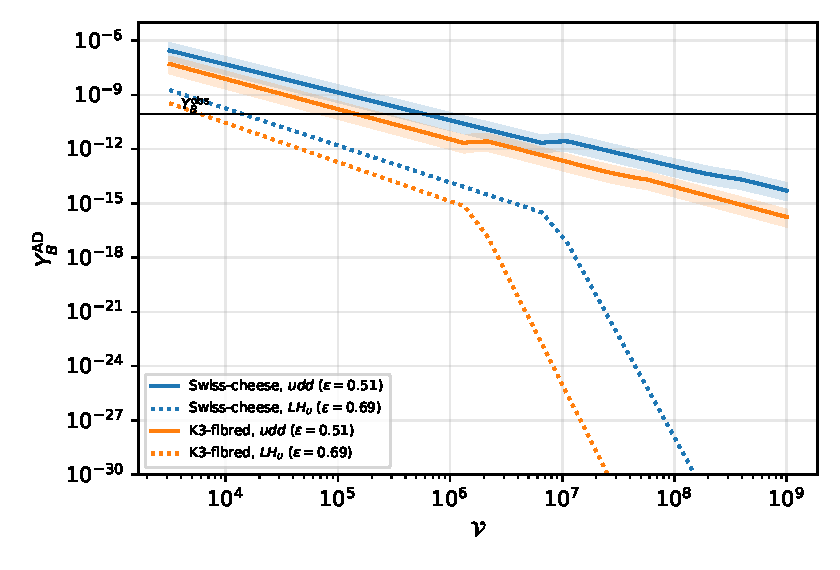
\includegraphics[width=.62\textwidth]{fig_AD.pdf}
\caption{Affleck--Dine yield in the explicit vacua: baryonic $udd$ direction (solid: benchmark $\epsilon=0.51$; band: median to maximal efficiency, $0.16$--$1.2$) and leptonic $LH_u$ (dotted, $\epsilon=0.69$) for Swiss-cheese (blue) and K3-fibred (orange) geometries. The horizontal line is the observed asymmetry.}\label{fig:AD}
\end{figure}
\begin{table}[t]
\centering\small
\begin{tabular}{c|cc}
\toprule
$m_{\rm AD}/m_{\rm mod}$ & Swiss, $\mathcal V_{\max}$ & K3, $\mathcal V_{\max}$\\
\midrule
$10^{-1}$ & $6.6\times10^{5}$ & $1.6\times10^{5}$ \\
$10^{-2}$ & $1.4\times10^{6}$ & $3.2\times10^{5}$ \\
$10^{-4}$ & $1.2\times10^{7}$ & $2.4\times10^{6}$ \\
$10^{-6}$ & $5.9\times10^{7}$ & $10.0\times10^{6}$ \\
\bottomrule
\end{tabular}
\caption{Case II ($m_{\rm AD}<m_{\rm mod}$, $udd$, $\epsilon=1$): maximal $\mathcal V$ as a function of the ratio of soft mass to modulus mass.}\label{tab:ad2}
\end{table}

\subsection{Numerical determination of the charge efficiency}\label{sec:adsim}
We integrate the field equations of \eqref{eq:adpot} in a matter-dominated background ($H=2/3t$, inflaton oscillations), the background in which the Hubble-induced terms exist in units $\phi=\MP f$, $\tau=m_{\rm AD}t$, $\mu=m_{\rm AD}/\MP$, $h=H/m_{\rm AD}$:
\begin{equation}
f''+3hf'+(1-ch^2)f+\frac{(n-1)\lambda^2}{\mu^2}|f|^{2n-4}f+\frac{\lambda}{\mu}\,f^{*\,n-1}\big(a\,e^{-i\alpha}+a_Hh\,e^{-i\alpha_H}\big)=0.\label{eq:adeom}
\end{equation}
The Hubble-induced $A$-term fixes the phase of the field during $H\gg m_{\rm AD}$, and CP violation is the misalignment $\delta=\alpha-\alpha_H$ between that phase and the low-energy $A$-term, which kicks the field when $H\sim m_{\rm AD}$. For $h\gg1$ the dynamics is scale free and has the exact attractor $f=R\,t^{-1/(n-2)}e^{i\theta_{\min}}$ with $n\theta_{\min}+\arg(a_{\rm tot})=\pi$, where $R$ solves $\big[p(p+1)-3\kappa p-c\kappa^2\big]R+(n-1)\lambda^2R^{2n-3}/\mu^2-\kappa\lambda a_HR^{n-1}/\mu=0$ with $p=1/(n-2)$ and $H=\kappa/t$ ($\kappa=2/3$ here); we start on this attractor with the exact velocity. Starting on an approximate tracking solution instead leaves transients that decay only as a slow power of $t$ and give $\epsilon$ varying by a factor two with the starting time; with the attractor, $\epsilon$ is independent of the starting $h\in[100,1600]$ to $3\times10^{-3}$. The comoving charge $Q=a^3\,i(\dot\phi^*\phi-\phi^*\dot\phi)$ is normalised to $a^3m_{\rm AD}|\phi_0|^2$ at $H=m_{\rm AD}$, defining $\epsilon$; it is constant after $h\lesssim0.1$ to $10^{-4}$, and independent of $\mu$.

For the benchmark $a=a_H=c=\lambda=1$, $\delta=\pi/2$ we find $|\epsilon|=0.51$ ($n=6$) and $0.69$ ($n=4$); a radiation background would give $0.52$ and $0.74$. Table~\ref{tab:adsim} shows the dependence on each parameter, and a scan of $162$ points ($c,a,a_H\in\{0.3,1,3\}$, six values of $\delta$) gives median $|\epsilon|=0.16$, 90th percentile $0.55$ and maximum $1.2$.
\begin{table}[t]
\centering\small
\begin{tabular}{l|ccc|cccc|ccc|ccc}
\toprule
 & \multicolumn{3}{c|}{$a$} & \multicolumn{4}{c|}{$\delta$} & \multicolumn{3}{c|}{$c$} & \multicolumn{3}{c}{$a_H$}\\
value & $0.3$ & $1$ & $3$ & $\tfrac\pi8$ & $\tfrac\pi4$ & $\tfrac\pi2$ & $\tfrac{3\pi}4$ & $0.3$ & $1$ & $3$ & $0.3$ & $1$ & $3$\\
\midrule
$|\epsilon|$ & $0.21$ & $0.51$ & $0.06$ & $0.10$ & $0.21$ & $0.51$ & $0.69$ & $0.54$ & $0.51$ & $0.42$ & $0.56$ & $0.51$ & $0.44$\\
\bottomrule
\end{tabular}
\caption{Charge efficiency for the $udd$ direction ($n=6$): one parameter varied at a time around the benchmark. The sign of $\epsilon$ is negative for $\delta\in(0,\pi)$ at the benchmark.}\label{tab:adsim}
\end{table}
We therefore adopt $|\epsilon|=0.51$ as the benchmark, the median $0.16$ as the typical value for a generic $A$-term, and $1.2$ as the ceiling in the scanned range; the ceiling gives the largest volume at which any $A$-term in that range can produce $Y_B^{\rm obs}$ (Table~\ref{tab:ad}).

\subsection{Relation to previous work}
Previous Affleck--Dine analyses in LVS considered late-time AD leptogenesis after double thermal inflation \cite{Choi:2012}, a regime in which the moduli are diluted by thermal inflation and the asymmetry is produced after the last inflationary stage. We consider the opposite ordering: the asymmetry is produced early, before the modulus oscillates, and is subsequently diluted by the modulus itself, which gives the closed form of Prop.~\ref{prop:AD}. The inputs we share with \cite{Choi:2012} agree: $m_{\phi_b}\sim m_{3/2}/\tau_b^{3/4}\sim\MP\mathcal V^{-3/2}$ up to logarithms, $\Gamma_{\phi_b\to2a_b}=m_{\phi_b}^3/48\pi\MP^2$, and the yield $n_\phi/s=\tfrac34T_R/m_\phi$ of a modulus decaying from domination; they also note that soft terms may be sequestered to $m_{\rm soft}\lesssim m_{\phi_b}$, which is our Case II.

\subsection{Assumptions and caveats}
(i) Case~I requires inflaton oscillations until $H\simeq m_{\rm AD}$ and reheating at $T_{\rm RH}\le T_{\rm AD}\simeq0.54\sqrt{m_{\rm AD}\MP}$; the yield scales as $T_{\rm RH}/T_{\rm AD}$ below that, so the windows are upper bounds. (ii) The displacement $|\phi_0|\gg T_{\rm AD}$ in the windows, so thermal-mass effects are subleading. (iii) The condensate can fragment into $Q$-balls in gravity-mediated scenarios; this changes the dynamics but not the total charge, and we do not analyse their stability, but for $m_{\rm AD}\gtrsim10^{9}$~GeV we expect them to decay well before BBN. (iv) With $m_{\rm AD}\gtrsim10^{9}$~GeV the low-energy theory is not supersymmetric, and the flat direction is a high-scale object; dark matter must then be supplied independently. (v) $c$, $\lambda$ and $r_i$ are parameters, with the effect of $c$ and $\lambda$ quantified in Prop.~\ref{prop:AD} and the efficiency $\epsilon$ computed in Sec.~\ref{sec:adsim}; the dependence on the A-term phase and strength is $\mathcal O(1)$ and its microscopic origin (the string-theory $A$-terms) is not derived.

\section{Discussion}\label{sec:disc}
\paragraph{What is established.} Given the Boltzmann system \eqref{eq:boltz}, \eqref{eq:washout} and the lattice rate \eqref{eq:rate}: the dilution law, the washout efficiencies, the equilibrium window, Prop.~\ref{prop:frame}, Prop.~\ref{prop:AD}, Thms.~\ref{thm:axion} and~\ref{thm:dm} (the first two are exact statements given their assumptions).

\paragraph{Limitations.} (1) The lattice parametrisation \eqref{eq:rate} has a factor $\sim5$ discontinuity at $T_c$; window edges near $T_c$ are uncertain by a few GeV, and the efficiencies $\eta_{B,L}$ by an $\mathcal O(1)$ factor from $c$ (the exponent in $\eta_L\propto T_R^4$ is robust since $f_{\rm win}\propto\Gamma/H\propto\Gamma^2$). (2) $g_*(T)$ is approximated near the QCD crossover. (3) The Swiss-cheese vacua are AdS (no uplift), which changes masses at the $\mathcal O(1)$ level relative to a de Sitter vacuum; the explicit vacua are for one geometry with $a$ treated as continuous and $W_0=A=1$; the decay width $\Gamma=c_\Gamma m^3/4\pi\MP^2$ is parametrised by $c_\Gamma$, which a specific visible-sector embedding would fix; varying $c_\Gamma$ over $[0.3,8]$ changes $\mathcal V_{\max}$ by a factor $\lesssim2$ (not the scalings). The CP-violating baryon number $\epsilon$ is not computed. (4) For K3-fibred geometries the string-loop potential is a conjecture based on torus computations and low-energy arguments \cite{Cicoli:2008}; we use the published coefficient sets and variations by factors of three, which give $c_f=0.7$--$17$ and hence a factor $\lesssim4$ uncertainty in $\mathcal V_{\max}$. (5) All bounds assume the lightest modulus dominates before decaying (Sec.~\ref{sec:bg}). (6) Thm.~\ref{thm:axion} assumes Chern--Simons-driven baryogenesis through sphalerons; mechanisms with direct baryon-violating couplings are covered in (d), and non-sphaleron axion mechanisms are not constrained. (7) We assume radiation-dominated physics for $T_{\rm gen}\sim131.7$~GeV is set by the sphaleron freeze-out; generation at higher $T$ is bounded more strongly through $T_R^{\min}\propto T_{\rm gen}$.

\paragraph{Outlook.} The main open question is the explicit volume-modulus branching ratios and CP phases (or, for AD, the $A$-term phase) in a concrete compactification, which would fix $\epsilon$ and turn the windows above into predictions; a second is the fate of the AD condensate under $Q$-ball fragmentation in a full supergravity treatment.

\ifx\codeurl\empty\else\paragraph{Code availability.} All figures, tables and numerical results can be reproduced with the code at \url{\codeurl}.\fi

\appendix
\section{Numerical method}\label{app:num}
We integrate \eqref{eq:boltz} and \eqref{eq:washout} in $N=\ln a$ with a stiff solver (Radau, $\mathrm{rtol}=10^{-9}$--$10^{-10}$, $\mathrm{atol}=10^{-35}$ for the asymmetries), initialised at $T=3$~TeV on the steady-state attractor $\rho_R=\tfrac65\Gamma\MP^2H$. The temperature is obtained by inverting $\rho_R=\frac{\pi^2}{30}g_*(T)T^4$ with $g_*(T)$ a log-linear interpolation through $(T/\text{GeV},g_*)=(10^{-4},10.75),(0.05,10.75),(0.2,50),(0.5,65),(1,75),(3,80),(10,86),(100,96),(170,106.75)$. $\mathcal D=S(\Tgen)/S$ is evaluated when $\rho_\phi/\rho_R<10^{-7}$.

\section{Susceptibility derivation}\label{app:xi}
With flavour-universal potentials $\mu_Q,\mu_L,\mu_H$ and $\mu_u=\mu_Q+\mu_H$, $\mu_d=\mu_Q-\mu_H$, $\mu_e=\mu_L-\mu_H$, hypercharge neutrality reads
\begin{equation}
n_g\Big[6\cdot\tfrac16\mu_Q+3\cdot\tfrac23\mu_u-3\cdot\tfrac13\mu_d-2\cdot\tfrac12\mu_L-\mu_e\Big]+2\cdot\tfrac12\cdot2\,\mu_H=0,
\end{equation}
(the Higgs term carries the bosonic factor $T^2/3$ versus $T^2/6$ for fermions), the sphaleron bias is $n_g(3\mu_Q+\mu_L)=\mu_{\rm CS}$, and $B-L=\tfrac13n_g(6\mu_Q+3\mu_u+3\mu_d)-n_g(2\mu_L+\mu_e)$ in units of $T^2/6$. Solving with $B-L=0$ gives $n_B=\tfrac{12}{79}T^2\mu_{\rm CS}$; solving with $\mu_{\rm CS}=0$ gives $B=\tfrac{28}{79}(B-L)$.

\section{Kähler metric of the blow-up modulus}\label{app:K}
For $K=-2\ln\mathcal V$ with $\mathcal V=\gamma(\tau_b^{3/2}-\tau_s^{3/2})$ and $\tau=\tfrac12(T+\bar T)$, $K_{s\bar s}=\tfrac14\partial_{\tau_s}^2K$. Expanding for $\tau_s^{3/2}\ll\tau_b^{3/2}$,
\begin{equation}
K=-2\ln(\gamma\tau_b^{3/2})+2\frac{\tau_s^{3/2}}{\tau_b^{3/2}}+\dots\ \Rightarrow\ K_{s\bar s}\simeq\frac{3\gamma}{8\sqrt{\tau_s}\,\mathcal V}.
\end{equation}
We verified this against the exact second derivative at $\mathcal V=1.5\times10^{14}$, $\tau_s=25.1$ (agreement to four digits), and verified numerically that the full supergravity potential with $W_0$ only reproduces the $\alpha'$ term $3\hat\xi W_0^2/4\mathcal V^3$ exactly (no-scale cancellation) for $\hat\xi=252$.

\section{Explicit vacuum computation}\label{app:vac}
With $\tau_i=\mathrm{Re}\,T_i$, $K_{i\bar j}=\tfrac14\partial_{\tau_i}\partial_{\tau_j}K$ and $K_i=\tfrac12\partial_{\tau_i}K$. For $\tau_s\ll\tau_b$ the potential reduces to three terms,
\begin{equation}
V\simeq\frac{\alpha}{\mathcal V}-\frac{\beta}{\mathcal V^2}+\frac{\delta}{\mathcal V^3},\quad\alpha=\frac{8\sqrt{\tau_s}}{3\gamma}(aA)^2e^{-2a\tau_s},\ \beta=4aAW_0\tau_se^{-a\tau_s},\ \delta=\frac{3\hat\xi W_0^2}{4},
\end{equation}
whose extremum in $\mathcal V$ requires $\beta^2\ge3\alpha\delta$, i.e.\ $\tau_s^{3/2}\ge3\hat\xi/8\gamma$, and lies at $\mathcal V=(\beta-\sqrt{\beta^2-3\alpha\delta})/\alpha$. We use the minimum of this reduced potential in $\tau_s$ as the starting point and then minimise the exact supergravity potential. Checks: (i) with $A=0$ the exact potential reproduces $3\hat\xi W_0^2/4\mathcal V^3$ (no-scale cancellation) to all digits; (ii) the three terms are reproduced numerically ($\alpha/\mathcal V=7.2\times10^{-40}$, $\beta/\mathcal V^2=1.1\times10^{-40}$ at $\mathcal V=1.5\times10^{14}$, $\tau_s=25.1$); (iii) $K_{s\bar s}$ agrees with App.~\ref{app:K}. Masses are the eigenvalues of $G^{-1}\partial^2V$ with $G=2\MP^2K_{i\bar j}$; the axion mass is $m_\rho^2=a^2\partial^2_\varphi V/2K_{s\bar s}$ with $\varphi=a\,\mathrm{Im}\,T_s$.

\section{K3-fibred Kähler geometry and explicit vacuum}\label{app:k3}
For $K=-2\ln\mathcal V$ with $\mathcal V=\alpha\sqrt{\tau_1}\tau_2-\gamma\tau_3^{3/2}$ and $\gamma\to0$ one has $K=-\ln\tau_1-2\ln\tau_2+\text{const}$, hence $K_{i\bar j}=\tfrac14\partial_{\tau_i}\partial_{\tau_j}K=\mathrm{diag}\big(1/4\tau_1^2,\,1/2\tau_2^2,\,0\big)$ (verified symbolically). Along the flat direction $\delta\tau_2/\tau_2=-\tfrac12\delta\tau_1/\tau_1$ the kinetic metric $G=2\MP^2K_{i\bar j}\delta\tau^i\delta\tau^j$ equals $\tfrac34\MP^2(\delta\ln\tau_1)^2$; along $\delta\tau_2/\tau_2=\delta\mathcal V/\mathcal V$ at fixed $\tau_1$ it equals $\MP^2(\delta\ln\mathcal V)^2$. For the explicit vacua we use the full Kähler metric of $K=-2\ln(\mathcal V+\hat\xi/2)$ with $\mathcal V=\alpha(\sqrt{\tau_1}\tau_2-\gamma\tau_3^{3/2})$, transformed with the Jacobian of $(\tau_1,\tau_2,\tau_3)\to(\tau_1,\mathcal V,\tau_3)$, $\tau_2=(\mathcal V/\alpha+\gamma\tau_3^{3/2})/\sqrt{\tau_1}$, and the masses are the eigenvalues of $G^{-1}\partial^2V$ with $G=2\MP^2K_{i\bar j}$ and $V$ multiplied by $g_se^{K_{cs}}/8\pi$.

\begin{thebibliography}{99}
\bibitem{Coughlan:1983ci} G.~D.~Coughlan et al., Phys.\ Lett.\ B \textbf{131} (1983) 59.
\bibitem{Banks:1993en} T.~Banks, D.~B.~Kaplan, A.~E.~Nelson, Phys.\ Rev.\ D \textbf{49} (1994) 779, hep-ph/9308292.
\bibitem{deCarlos:1993jw} B.~de~Carlos, J.~A.~Casas, F.~Quevedo, E.~Roulet, Phys.\ Lett.\ B \textbf{318} (1993) 447, hep-ph/9308325.
\bibitem{Balasubramanian:2005zx} V.~Balasubramanian, P.~Berglund, J.~P.~Conlon, F.~Quevedo, JHEP \textbf{03} (2005) 007, hep-th/0502058.
\bibitem{Conlon:2005ki} J.~P.~Conlon, F.~Quevedo, K.~Suruliz, JHEP \textbf{08} (2005) 007, hep-th/0505076.
\bibitem{Choi:2012} K.~Choi, W.-I.~Park, C.~S.~Shin, JCAP \textbf{03} (2013) 011, arXiv:1211.3755.
\bibitem{Cicoli:2012} M.~Cicoli, J.~P.~Conlon, F.~Quevedo, Phys.\ Rev.\ D \textbf{87} (2013) 043520, arXiv:1208.3562.
\bibitem{Higaki:2012} T.~Higaki, F.~Takahashi, JHEP \textbf{11} (2012) 125, arXiv:1208.3563.
\bibitem{Cicoli:2008} M.~Cicoli, C.~P.~Burgess, F.~Quevedo, JCAP \textbf{03} (2009) 013, arXiv:0808.0691.
\bibitem{DLR:2000} S.~Davidson, M.~Losada, A.~Riotto, Baryogenesis at low reheating temperatures, arXiv:hep-ph/0001301.
\bibitem{GHKO:2026} M.~A.~G.~Garcia, S.~E.~Henrich, W.~Ke, K.~A.~Olive, Leptogenesis and low reheating temperatures, arXiv:2607.08663.
\bibitem{McDonald:1991} J.~McDonald, Phys.\ Rev.\ D \textbf{43} (1991) 1063.
\bibitem{Giudice:2000} G.~F.~Giudice, E.~W.~Kolb, A.~Riotto, Phys.\ Rev.\ D \textbf{64} (2001) 023508, arXiv:hep-ph/0005123.
\bibitem{Co:2019} R.~T.~Co, K.~Harigaya, Phys.\ Rev.\ Lett.\ \textbf{124} (2020) 111602, arXiv:1910.02080.
\bibitem{Snowmass:2022} New Ideas in Baryogenesis: A Snowmass White Paper, arXiv:2203.05010.
\bibitem{Asadi:2025} P.~Asadi, D.~Cyncynates, S.~Gori, Axiverse Baryogenesis, arXiv:2511.15794.
\bibitem{DRT:2014} M.~D'Onofrio, K.~Rummukainen, A.~Tranberg, Phys.\ Rev.\ Lett.\ \textbf{113} (2014) 141602, arXiv:1404.3565.
\bibitem{DRT:2012} M.~D'Onofrio, K.~Rummukainen, A.~Tranberg, JHEP \textbf{08} (2012) 123, arXiv:1207.0685.
\end{thebibliography}
\end{document}
